\documentclass[a4paper,adobefonts,11pt,UTF8]{book}

%type chinese characters
\usepackage{ctex}

%generate index of book
\usepackage{makeidx}

%modify the headheight at least 13.5pt
\usepackage[headheight=13.6pt]{geometry}

%
\usepackage{fontspec}

%unicode
\usepackage{xunicode}

%
\usepackage{xltxtra}

%mathematics package
\usepackage{amsmath}

%mathematics symbols
\usepackage{amssymb}

%origin print package
\usepackage{verbatim}

%draw graphics use tikz and so on.
\usepackage{graphicx}

%set graphics path which used in the book.
\graphicspath{{../img/}}

%colorful table
\usepackage{colortbl}

%set color use origin name directly.
\usepackage[svgnames,table]{xcolor}

%
\usepackage[figuresright]{rotating}

% generate longtable which could across pages.
\usepackage{longtable}

%
\newcommand\mgape[1]{\gape{$\vcenter{\hbox{#1}}$}}

%
\usepackage{array}

%
\usepackage{makecell}

%
\usepackage{ulem}

%
\usepackage{color}

% draw graphics use tikz package
\usepackage{tikz}

%
\usepackage{listings}
\lstset{
  basicstyle=\ttfamily,
  showstringspaces=false,
  commentstyle=\color{red},
  keywordstyle=\color{blue},
  columns=flexible,
  backgroundcolor=\color{lightgray},
  extendedchars=true,
  basicstyle=\footnotesize\ttfamily,
  showstringspaces=false,
  showspaces=false,
  numbers=left,
  numberstyle=\footnotesize,
  numbersep=9pt,
  tabsize=2,
  breaklines=true,
  showtabs=false,
  captionpos=b
}

%
\usepackage{bashful}

%set book information including bookmarksnumbered,pdfencoding,
%pdfauthor,pdfpagelayout,breaklinks,colorlinks,linkcolor,
%urlcolor,and so on.
\usepackage[bookmarksnumbered,pdfencoding=auto,pdfauthor={穷屌丝联盟},pdfpagelayout=TwoPageRight,breaklinks,colorlinks,linkcolor=RoyalBlue,urlcolor=blue,colorlinks=true]{hyperref}

%add more list types.
\usepackage{paralist}

%set page styles
\usepackage{fancyhdr}

\pagestyle{fancy}
\fancyhf{}
\fancyhead[LE,RO]{\thepage}
\fancyhead[RE]{\leftmark}
\fancyhead[RO]{\rightmark}
\fancypagestyle{plain}{
  \fancyhf{}
  \renewcommand{\headrulewidth}{0pt}
}


%titlepage \titleGM
\newcommand*{\plogo}{\fbox{$\mathcal{PL}$}} % Generic publisher logo
%--------------------------------------------------------------------
% TITLE PAGE
%--------------------------------------------------------------------

\newcommand*{\titleGM}{\begingroup % Create the command for including the title page in the document
\hbox{ % Horizontal box
\hspace*{0.2\textwidth} % Whitespace to the left of the title page
\rule{1pt}{\textheight} % Vertical line
\hspace*{0.05\textwidth} % Whitespace between the vertical line and title page text
\parbox[b]{0.75\textwidth}{ % Paragraph box which restricts text to less than the width of the page
{\noindent\Huge\bfseries A Collection of \\[0.5\baselineskip] PHP}\\[2\baselineskip] % Title
{\large \textit{PHP}}\\[4\baselineskip] % Tagline or further description
{\Large \textsc{theqiong.com}} % Author name

\vspace{0.5\textheight} % Whitespace between the title block and the publisher
{\noindent 穷屌丝联盟}\\[\baselineskip] % Publisher and logo
}}
\endgroup}
%


%lstlisting[language=JavsScript]
% Taken from Lena Herrmann at 
% http://lenaherrmann.net/2010/05/20/javascript-syntax-highlighting-in-the-latex-listings-package
\definecolor{lightgray}{rgb}{.9,.9,.9}
\definecolor{darkgray}{rgb}{.4,.4,.4}
\definecolor{purple}{rgb}{0.65,0.12,0.82}

%lstlisting package -----------
% JavaScript
%------------------------------
\lstdefinelanguage{JavaScript}
{
  keywords={typeof,new,ture,false,catch,function,return,null,switch,var,if,in,while,do,else,case,break},
  keywordstyle=\color{blue}\bfseries,
  ndkeywords={class,export,boolean,throw,implements,import,this},
  ndkeywordstyle=\color{darkgray}\bfseries,
  identifierstyle=\color{black},
  sensitive=false,
  comment=[l]{//},
  morecomments[s]{/*}{*/},
  commentstyle=\color{purple}\ttfamily,
  stringstyle=\color{red}\ttfamily,
  morestring=[b]',
  morestring=[b]"
}

\lstdefinelanguage{Scheme}
{morekeywords={,lambda, cond, case, display, let, import, quote, quasiquote, unquote,
define, begin, newline, if, list, apply, null?, car, cdr, or, not, and, for-each, 
make-vector, vector-length, vector-ref, vector-set!, eqv?, eq?, equal?, else, set!, 
define-record-type, fields, mutable, immutable, assert, parent, with-exception-handler, }
sensitive=false,
morecomment=[l]{;},
morecomment=[s]{/*}{*/},
morestring=[b]",
}

\lstdefinelanguage{CSS}{
  morekeywords={accelerator,azimuth,background,background-attachment,
    background-color,background-image,background-position,
    background-position-x,background-position-y,background-repeat,
    behavior,border,border-bottom,border-bottom-color,
    border-bottom-style,border-bottom-width,border-collapse,
    border-color,border-left,border-left-color,border-left-style,
    border-left-width,border-right,border-right-color,
    border-right-style,border-right-width,border-spacing,
    border-style,border-top,border-top-color,border-top-style,
    border-top-width,border-width,bottom,caption-side,clear,
    clip,color,content,counter-increment,counter-reset,cue,
    cue-after,cue-before,cursor,direction,display,elevation,
    empty-cells,filter,float,font,font-family,font-size,
    font-size-adjust,font-stretch,font-style,font-variant,
    font-weight,height,ime-mode,include-source,
    layer-background-color,layer-background-image,layout-flow,
    layout-grid,layout-grid-char,layout-grid-char-spacing,
    layout-grid-line,layout-grid-mode,layout-grid-type,left,
    letter-spacing,line-break,line-height,list-style,
    list-style-image,list-style-position,list-style-type,margin,
    margin-bottom,margin-left,margin-right,margin-top,
    marker-offset,marks,max-height,max-width,min-height,
    min-width,-moz-binding,-moz-border-radius,
    -moz-border-radius-topleft,-moz-border-radius-topright,
    -moz-border-radius-bottomright,-moz-border-radius-bottomleft,
    -moz-border-top-colors,-moz-border-right-colors,
    -moz-border-bottom-colors,-moz-border-left-colors,-moz-opacity,
    -moz-outline,-moz-outline-color,-moz-outline-style,
    -moz-outline-width,-moz-user-focus,-moz-user-input,
    -moz-user-modify,-moz-user-select,orphans,outline,
    outline-color,outline-style,outline-width,overflow,
    overflow-X,overflow-Y,padding,padding-bottom,padding-left,
    padding-right,padding-top,page,page-break-after,
    page-break-before,page-break-inside,pause,pause-after,
    pause-before,pitch,pitch-range,play-during,position,quotes,
    -replace,richness,right,ruby-align,ruby-overhang,
    ruby-position,-set-link-source,size,speak,speak-header,
    speak-numeral,speak-punctuation,speech-rate,stress,
    scrollbar-arrow-color,scrollbar-base-color,
    scrollbar-dark-shadow-color,scrollbar-face-color,
    scrollbar-highlight-color,scrollbar-shadow-color,
    scrollbar-3d-light-color,scrollbar-track-color,table-layout,
    text-align,text-align-last,text-decoration,text-indent,
    text-justify,text-overflow,text-shadow,text-transform,
    text-autospace,text-kashida-space,text-underline-position,top,
    unicode-bidi,-use-link-source,vertical-align,visibility,
    voice-family,volume,white-space,widows,width,word-break,
    word-spacing,word-wrap,writing-mode,z-index,zoom},
  morestring=[s]{:}{;},
  sensitive,
  morecomment=[s]{/*}{*/}
}


\setmainfont[Mapping=tex-text]{Minion Pro}

\makeindex


\title{PHP Notes}
\author{穷屌丝联盟}
\date{\today}








\begin{document}

\begin{titlepage}
\addcontentsline{toc}{part}{Cover}

\pagestyle{empty} % Removes page numbers

\titleGM % This command includes the title page


\end{titlepage}

\maketitle
\tableofcontents
\listoffigures
\listoftables
\printindex

\part{Introduction}

PHP\cite{php_wiki} is a server-side scripting language designed for web development but also used as a general-purpose programming language. PHP is now installed on more than 244 million websites and 2.1 million web servers. Originally created by Rasmus Lerdorf in 1995, the reference implementation of PHP is now produced by The PHP Group. While PHP originally stood for Personal Home Page, it now stands for PHP: Hypertext Preprocessor, a recursive acronym.

PHP\footnote{PHP:Hypertext Preprocessor,递归命名。}(Hypertext Preprocessor,超文本预处理器)是一种开源的通用计算机脚本语言,尤其适用于网络开发并可嵌入HTML中使用,现在大多数的Web主机都提供 PHP 的支持,而且使用PHP完全是免费的。

PHP code is interpreted by a web server with a PHP processor module, which generates the resulting web page: PHP commands can be embedded directly into an HTML source document rather than calling an external file to process data. It has also evolved to include a command-line interface capability and can be used in standalone graphical applications.

对于大多数的服务器,PHP 提供了一个模块,而且PHP 支持 CGI 标准,因而使得 PHP 能够作为 CGI 处理器来工作。作为一种免费的,并且使用广泛的创建动态交互性站点的强有力的服务器端脚本语言,对于像微软 ASP 这样的竞争者来说,PHP 无疑是另一种高效率的选项。

PHP is free software released under the PHP License, which is incompatible with the GNU General Public License (GPL) due to restrictions on the usage of the term PHP. PHP can be deployed on most web servers and also as a standalone shell on almost every operating system and platform, free of charge.



PHP最初由勒多夫在1995年开始开发,现在PHP的标准由PHP Group和开放源代码社区维护。PHP以PHP License作为许可协议,不过因为这个协议限制了PHP名称的使用,所以和开放源代码许可协议GPL不兼容。

PHP 文件的文件后缀是``.php"、``.php3" 或 ``.phtml",其中``.php"是 PHP 的默认扩展名,所有以 .php 结尾的文件都将由 PHP 来处理。在支持PHP的服务器上,只需要建立 .php 文件,并把它们放置到Web目录中,服务器将自动解析这些文件,不用编译任何东西,也不用安装任何其它的工具,仅仅只需把这些使用了 PHP 的文件想象成简单的 HTML 文件,其中只不过多了一种新的标识符,在这里可以做各种各样的事情。

PHP的主要目标是允许网络开发人员快速编写动态页面,其语法借鉴了C、Java和Perl等流行计算机语言的特点,易于一般程序员学习。使用 PHP 的一大好处是它对于初学者来说极其简单,同时也给专业的程序员提供了各种高级的特性,而且尽管 PHP 的开发是以服务端脚本为目的,但事实上其功能远不局限与此,PHP也被用于其他很多领域。


\zihao{6}



\begin{longtable}{|m{16pt}|m{20pt}|m{35pt}|m{300pt}|}

%head
\multicolumn{4}{r}{}
\tabularnewline\hline
主要\newline 版本	&次要\newline 版本	&发布日期	&说明
\endhead
%endhead

%firsthead
\caption{PHP版本历程}\\
\hline
主要\newline 版本	&次要\newline 版本	&发布日期	&说明
\endfirsthead
%endfirsthead

%foot
\multicolumn{4}{r}{}
\endfoot
%

%lastfoot
\endlastfoot
%endlastfoot

\hline
1.0		&1.0.0	&1995-06-08	&正式名称为``Personal Home Page Tools (PHP Tools)",第一次使用了``PHP"的名字。\\
\hline
2.0		&2.0.0	&1996-04-16	&针对PHP 1.0的改进版,速度更快、体积更小,更容易产生动态网页。\\
\hline
3.0		&3.0.0	&1998-06-06	&开发方式改成多人共同参与。Zeev Suraski和Andi Gutmans为了这个版本重写了剖析引擎。\\
\hline
\multirow{7}{40pt}{4.0}		&4.0.0	&2000-05-22	&改成以Zend引擎作为语法分析器,具有两阶段剖析/标签剖析系统等先进功能。\\ \cline{2-4}

		&4.1.0	&2001-12-10	&加入``超全局变量"(superglobals)功能,包含了\$\_GET、\$\_POST、\$\_SESSION等。\\  \cline{2-4}

		&4.2.0	&2002-04-22	&默认取消register\_globals功能。从网络接收的数据将不会设置成全局变量,增加程序安全性。\\ \cline{2-4}

		&4.3.0	&2002-12-27	&加入命令行可执行文件,称为CLI。\\ \cline{2-4}

		&4.4.0	&2005-07-11	&Added man pages for phpize and php-config scripts.\\ \cline{2-4}

		&4.4.8	&2008-01-03	&一些安全性的增强。曾可能为PHP 4的最后版本。若有必要,提供安全性更新到2008-08-08。\\ \cline{2-4}

		&4.4.9	&2008-08-07	&更多安全性增强和问题修补。PHP 4.4系列的最后版本。\\ \cline{2-4}
\hline
\multirow{18}{40pt}{5.0}		&5.0.0	&2004-07-13	&Zend Engine II with a new object model.\\ \cline{2-4}

		&5.1.0	&2005-11-24	&Performance improvements with introduction of compiler variables in re-engineered PHP Engine.\\ \cline{2-4}

		&5.2.0	&2006-11-02	&默认打开``过滤"的扩展。\\ \cline{2-4}

		&5.2.8	&2008-12-08	&emergent bug fix。\\ \cline{2-4}

		&5.2.9	&2009-02-26	&解决了5.2.*的超过了50多个错误和多个安全问题,增加了稳定性。\\ \cline{2-4}

		&5.2.10&2009-06-18	&这个版本修正了大量的bug和安全漏洞,并升级了时区数据库。\\ \cline{2-4}

		&5.2.17&2011-01-06	&修正了一个浮点数转化的Bug。\\ \cline{2-4}

		&5.3.0	&2009-06-30	&支持命名空间;\newline 使用XMLReader和XMLWriter增强XML支持;\newline 支持SOAP,延迟静态绑定,跳转标签(有限的goto), 闭包,Native PHP archives。\\ \cline{2-4}

		&5.3.3	&2010-07-22	&使用命名空间的类中,与类同名的成员函数不再作为构造函数。\\ \cline{2-4}

		&5.3.6	&2011-03-17	&修正一系列Bug。\\ \cline{2-4}

		&5.3.10&2012-02-02	&修正了Stefan Esser报告的任意远程代码执行漏洞,CVE-2012-0830。\\ \cline{2-4}

		&5.4.0	&2012-03-01	&支持Trait、简短数组表达式。\newline 移除了register\_globals, safe\_mode, allow\_call\_time\_pass\_reference, session\_register(), session\_unregister(), magic\_quotes以及session\_is\_registered()。\newline 加入了内建的Web服务器。\newline 增强了性能,减小内存使用量。\\ \cline{2-4}
\hline
6.0		&6.0.0	&	&支持Unicode;移除ereg扩展;\newline 内置Alternative PHP Cache;\newline 移除mime\_magic和重写fileinfo()以更好地支持MIME。\newline 部分PHP 6特性已加入至PHP 5.3.0(命名空间,延迟静态绑定,lambda函数,闭包,goto)和5.4.0(traits,闭包重绑定)中。\\ 
\hline
\end{longtable}



\zihao{5}

PHP含有一个彩蛋: 在PHP网址的后面加上特殊的字符串\footnote{?=PHPE9568F36-D428-11d2-A769-00AA001ACF42}会出现PHP的标志,而且PHP版本的不同,标志也会不一样。

PHP类似 ASP,两者都是服务器端的脚本语言,但是PHP可以在多数的服务器和操作系统上运行,包括 Linux、Unix 的各种变种(HP-UX、Solaris 和 OpenBSD等)、Microsoft Windows、Mac OS X、RISC OS 等。今天,PHP已经支持了大多数的 Web服务器,包括 Apache、Microsoft Internet Information Server(IIS)、Personal Web Server(PWS)、Netscape 以及 iPlant server、Oreilly Website Pro Server、Caudium、Xitami、OmniHTTPd 等。



PHP的应用范围相当广泛,尤其是在网页程序的开发上,PHP 文件可包含文本、HTML 标签以及脚本,但是PHP的用途并不局限于输出 HTML。PHP 还能被用来动态输出图像、PDF 文件甚至 Flash 动画(使用 libswf 和 Ming)。PHP还能够非常简便的输出文本,例如 XHTML 以及任何其它形式的 XML 文件,PHP 能够自动生成这些文件,然后通过在服务端开辟出一块动态内容的缓存从而直接把它们打印出来,或者将它们存储到文件系统中。







PHP 具有极其有效的文本处理特性,包括 Perl 兼容正则表达式(PCRE)以及许多扩展和工具可用于解析和访问 XML 文档。PHP 将所有的 XML 功能标准化于坚实的 libxml2 扩展,并且还增加了 SimpleXML,XMLReader 以及 XMLWriter 支持以扩充其功能。另外,PHP还有很多其它有趣的扩展库,以及一些附加的 PECL 扩展。






使用 PHP,除了可以自由地选择操作系统和Web服务器之外,还可以在开发时选择使用过程和面向对象,或者两者混合的方式来开发。尽管 PHP 4 不支持 OOP 所有的标准,但很多代码仓库和大型的应用程序(包括 PEAR 库)仅使用 OOP 代码来开发。后来PHP 5 弥补了 PHP 4 的这一弱点,引入了完全的对象模型。

另外,PHP 最强大最显著的特性之一,是它支持很大范围的数据库,包括MySQL、Informix、Oracle、Sybase、Solid、PostgreSQL、Generic ODBC 等。使用任何针对某数据库的扩展(例如 mysql)编写数据库支持的网页非常简单,或者使用抽象层如 PDO,或者通过 ODBC 扩展连接到任何支持 ODBC 标准的数据库。其它一些数据库也可能会用 cURL 或者 sockets,例如 CouchDB。



PHP 还支持利用诸如 LDAP、IMAP、SNMP、NNTP、POP3、HTTP、COM(Windows 环境)等不计其数的协议的服务,还可以开放原始网络端口,使得任何其它的协议能够协同工作。PHP 支持和所有Web开发语言之间的 WDDX 复杂数据交换。关于相互连接,PHP 已经支持了对 Java 对象的即时连接,并且可以透明地将其用作 PHP 对象。









\chapter{History}


PHP development began in 1994 when the developer Rasmus Lerdorf wrote a series of Common Gateway Interface (CGI) Perl scripts, which he used to maintain his personal homepage. The tools performed tasks such as displaying his résumé and recording his web traffic. He rewrote these scripts in C for performance reasons, extending them to add the ability to work with web forms and to communicate with databases, and called this implementation "Personal Home Page/Forms Interpreter" or PHP/FI. PHP/FI could be used to build simple, dynamic web applications. Lerdorf initially announced the release of PHP/FI as "Personal Home Page Tools (PHP Tools) version 1.0" publicly to accelerate bug location and improve the code, on the comp.infosystems.www.authoring.cgi Usenet discussion group on June 8, 1995. This release already had the basic functionality that PHP has as of 2013. This included Perl-like variables, form handling, and the ability to embed HTML. The syntax resembled that of Perl but was simpler, more limited and less consistent. A development team began to form and, after months of work and beta testing, officially released PHP/FI 2 in November 1997.


Zeev Suraski and Andi Gutmans rewrote the parser in 1997 and formed the base of PHP 3, changing the language's name to the recursive acronym PHP: Hypertext Preprocessor. Afterwards, public testing of PHP 3 began, and the official launch came in June 1998. Suraski and Gutmans then started a new rewrite of PHP's core, producing the Zend Engine in 1999. They also founded Zend Technologies in Ramat Gan, Israel.

On May 22, 2000, PHP 4, powered by the Zend Engine 1.0, was released. As of August 2008 this branch reached version 4.4.9. PHP 4 is no longer under development nor will any security updates be released.

On July 13, 2004, PHP 5 was released, powered by the new Zend Engine II. PHP 5 included new features such as improved support for object-oriented programming, the PHP Data Objects (PDO) extension (which defines a lightweight and consistent interface for accessing databases), and numerous performance enhancements. In 2008 PHP 5 became the only stable version under development. Late static binding had been missing from PHP and was added in version 5.3.

\vspace{-10pt}

\zihao{6}

\begin{longtable}{|m{25pt}|m{40pt}|m{60pt}|m{240pt}|}
%head
\multicolumn{4}{r}{}
\tabularnewline\hline
Version	&Release date	&Supported until	&Notes
\endhead
%endhead

%firsthead
\caption{PHP Release history}\\
\hline
Version	&Release date	&Supported until	&Notes
\endfirsthead
%endfirsthead

%foot
\multicolumn{4}{r}{}
\endfoot
%

%lastfoot
\endlastfoot
%endlastfoot

\hline
1.0	&1995-06-08		&						&Officially called "Personal Home Page Tools (PHP Tools)". 
												\newline This is the first use of the name "PHP".\\
\hline
2.0	&1997-11-01		&						&																								\\
\hline		
3.0	&1998-06-06		&2000-10-20			&Development moves from one person to multiple developers. 
												\newline Zeev Suraski and Andi Gutmans rewrite the base for this version.\\
\hline
4.0	&2000-05-22		&2001-01-23			&Added more advanced two-stage parse/execute tag-parsing system called the Zend engine.\\
\hline
4.1	&2001-12-10		&2002-03-12			&Introduced 'superglobals' (\$\_GET, \$\_POST, \$\_SESSION, etc.)\\
\hline
4.2	&2002-04-22		&2002-09-06			&Disabled register\_globals by default. 
												\newline Data received over the network is not inserted directly into the global namespace anymore, closing possible security holes in applications.\\
\hline
4.3	&2002-12-27		&2005-03-31			&Introduced the command-line interface (CLI), to supplement the CGI.\\
\hline
4.4	&2005-07-11		&2008-08-07			&Added man pages for phpize and php-config scripts.\\
\hline
5.0	&2004-07-13		&2005-09-05			&Zend Engine II with a new object model.\\
\hline
5.1	&2005-11-24		&2006-08-24			&Performance improvements with introduction of compiler variables in re-engineered PHP Engine. 
												\newline Added PHP Data Objects (PDO) as a consistent interface for accessing databases.\\
\hline
5.2	&2006-11-02		&2011-01-06			&Enabled the filter extension by default. Native JSON support.\\
\hline
5.3	&2009-06-30		&2014-07				&Namespace support; 
												\newline Late static bindings, Jump label (limited goto), Native closures, Native PHP archives (phar), garbage collection for circular references, improved Windows support, sqlite3, mysqlnd as a replacement for libmysql as underlying library for the extensions that work with MySQL, fileinfo as a replacement for mime\_magic for better MIME support, the Internationalization extension, and deprecation of ereg extension.\\
\hline
5.4	&2012-03-01		&3 years after release	&Trait Support, short array syntax support. 
												\newline Removed items: register\_globals, safe\_mode, allow\_call\_time\_pass\_reference, session\_register(), session\_unregister() and session\_is\_registered(). 
												\newline Built-in web server.
												\newline Several improvements to existing features, performance and reduced memory requirements.\\
\hline
5.5	&2013-06-20		&3 years after release	&Support for generators, finally blocks for exceptions handling, Zend Optimizer+ bundled in official distribution.\\
\hline
5.6	&No date set		&No date set			&Internal operator overloading, GMP changes\\
\hline
6	&No date set		&No date set			&The development of PHP 6 has been delayed because the developers have decided the current approach to handling of instance Unicode is not a good one, and are considering alternate ways in the next version of PHP.
												\newline The updates that were intended for PHP 6 were added to PHP 5.3.0 (namespace support, late static bindings, lambda functions, closures, goto) and 5.4.0 (traits, closure rebinding) instead.\\
\hline

\end{longtable}

\vspace{-10pt}


Beginning on June 28, 2011, the PHP Group began following a timeline for when new versions of PHP will be released. Under this timeline, at least one release should occur every month. Once per year, a minor release should occur which can include new features. Every minor release should at least have 2 years of security and bug fixes, followed by at least 1 year of only security fixes, for a total of a 3 year release process for every minor release. No new features (unless small and self-contained) will be introduced into a minor release during the 3-year release process.


\zihao{5}


A new major version has been under development alongside PHP 5 for several years. This version was originally planned to be released as PHP 6 as a result of its significant changes, which included plans for full Unicode support. However, Unicode support took developers much longer to implement than originally thought, and the decision was made in March 2010 to move the project to a branch, with features still under development moved to trunk.

Changes in the new code include the removal of \texttt{register\_globals}, magic quotes, and safe mode. The reason for the removals was that \texttt{register\_globals} had opened security holes by intentionally allowing runtime data injection, and the use of magic quotes had an unpredictable nature. Instead, to escape characters, magic quotes may be replaced with the \texttt{addslashes()} function, or more appropriately an escape mechanism specific to the database vendor itself like \texttt{mysql\_real\_escape\_string()} for MySQL. Functions that will be removed in future versions and have been deprecated in PHP 5.3 will produce a warning if used.

PHP interpreters are available on the most of existing 32-bit and 64-bit operating systems, through building binaries from the PHP sources. For the PHP versions 5.3 and 5.4, the only available Microsoft Windows binary distributions were 32-bit x86 builds, requiring Windows 32-bit compatibility mode while using Internet Information Services (IIS) on a 64-bit Windows platform. PHP version 5.5 made the 64-bit x86-64 builds available for Microsoft Windows.

PHP最初是拉斯姆斯·勒多夫为了要维护个人网页,而用c语言开发的一些用以取代原先使用的Perl程序的CGI工具程序集。这些工具程序用来显示拉斯姆斯·勒多夫的个人履历以及统计网页流量。他将这些程序和一些窗体解释器集成起来,称为PHP/FI。PHP/FI可以和数据库连接,产生简单的动态网页程序。

拉斯姆斯·勒多夫在1995年6月8日将PHP/FI公开发布,希望可以通过社区来加速程序开发与查找错误。这个发布的版本命名为PHP 2,已经有今日PHP的一些雏型,像是类似Perl的变量命名方式、窗体处理功能、以及嵌入到HTML中运行的能力。程序语法上也类似Perl,有较多的限制,不过更简单、更有弹性。

1997年,Zeev Suraski和Andi Gutmans重写了PHP的语法分析器,这成为了PHP 3的基础,而PHP也在这个时候改称为PHP: Hypertext Preprocessor。开发团队在1997年11月发布了PHP/FI 2,随后就开始PHP 3的开放测试,1998年6月正式发布PHP 3。Zeev Suraski和Andi Gutmans在PHP 3发布后开始改写PHP的核心,这个在1999年发布的语法分析器称为Zend Engine,他们也在以色列的Ramat Gan成立了Zend Technologies来管理PHP的开发。

在2000年5月22日,以Zend Engine 1.0为基础的PHP 4正式发布,2004年7月13日发布了PHP 5,PHP 5使用了第二代的Zend Engine,而且PHP包含了许多新特色,比如强化的面向对象功能、引入PDO以及许多性能上的增强。从2008年开始,PHP 5成为了PHP唯一维护中的稳定版本,PHP 4已经不会继续更新,以鼓励用户转移到PHP 5。

PHP 6的开发也正在进行中,主要的改进有移除\texttt{register\_globals}、magic quotes和Safe mode的功能。


要查看当前PHP信息,可以通过网页或者命令行,其中通过网页可以直观的显示。

\begin{lstlisting}[language=PHP]
<?php
	phpinfo();
?>
\end{lstlisting}

或者在命令行中输入如下的命令:

\begin{lstlisting}[language=bash]
php -i
//or
php -r 'phpinfo();'
\end{lstlisting}

调用函数 \texttt{phpinfo()}可以得到很多有关当前系统的有用信息,例如预定义变量、已经加载的 PHP 模块和配置信息。为了移除敏感信息,比如AUTH\_USER和AUTH\_PASSWORD,可以修改代码如下:

\begin{lstlisting}[language=PHP]
<?php
  // start output buffering
  ob_start();
  
  // send phpinfo content
  phpinfo();
  
  // get phpinfo content
  $html = ob_get_contents();
  
  // flush the output buffer
  ob_end_clean();
  
  // remove auth data
  if(isset($_SERVER['AUTH_USER']))
    $html = str_replace($_SERVER['AUTH_USER'], '<i>no value</i>',$html);
  if(isset($_SERVER['AUTH_PASSWORD']))
    $html = str_replace($_SERVER['AUTH_PASSWORD'], '<i>no value</i>', $html);
  echo $html;
?>
\end{lstlisting}

为了比较上述两种方法的异同,可以在一个页面中同时运行这两个测试页面:

\begin{lstlisting}[language=HTML]
<html>
  <frameset cols="50%,50%">
    <frame src="phptest.php">
    <frame src="phpinfo.php">
  </frameset>
</html>
\end{lstlisting}



















\chapter{Compatibility}

现在,PHP 已经发展成为一种流行的脚本语言,可以在很多公共的资源里找到可以在自己的脚本中重新利用的代码。

PHP 语言的开发者为向下兼容性下了很多功夫,因此在新版本的 PHP 下,老版本的代码应该可以在不作任何改动的情况下(理想地)运行。不过实际上,还是必须对老的代码做一些改动。

有可能影响到老版本的代码的最重要的两点改动分别是:

\begin{compactitem}
\item 取消了旧的 \texttt{\$HTTP\_*\_VARS}数组(在函数或者方法中原本是全局变量)。

\end{compactitem}

PHP 4.1.0 版本引入了如下超全局数组变量:

\begin{compactitem}
\item \texttt{\$\_GET}
\item \texttt{\$\_POST}
\item \texttt{\$\_COOKIE}
\item \texttt{\$\_SERVER}
\item \texttt{\$\_FILES}
\item \texttt{\$\_ENV}
\item \texttt{\$\_REQUEST}
\item \texttt{\$\_SESSION}
\end{compactitem}

老的 \texttt{\$HTTP\_*\_VARS}数组,诸如 \texttt{\$HTTP\_POST\_VARS}等,从 PHP 3 就已经开始使用,它们仍然存在。


自 PHP 5.0.0 起, 用 \texttt{register\_long\_arrays}设置选项可禁用 长类型的 PHP 预定义变量数组。


\begin{compactitem}
\item 外部变量不再被默认注册为全局变量。也就是说,从 PHP 4.2.0 版开始,php.ini 中的设置选项 \texttt{register\_globals}默认值变成了\texttt{off}。

\end{compactitem}

建议用以上提到的超全局数组变量来访问这些值。但可能老的脚本、书籍以及教程都可能建立在该设置为\texttt{on} 的基础上。

如果该选项被设置为\texttt{on},则可以在 \url{http://www.example.com/foo.php?id=42}中直接使用变量 \texttt{\$id}。但不管被设置为 \texttt{on}还是\texttt{off},\texttt{\$\_GET['id']}一直有效。







\chapter{Syntax}


\section{Basic language constructs}


The PHP syntax and semantics are the format (syntax) and the related meanings (semantics) of the text and symbols in the PHP programming language. They form a set of rules that define how a PHP program can be written and interpreted. PHP is a procedural and object-oriented language for coding webpage markup text to be transformed into HTML format.


Each PHP statement is terminated by semicolon ("\texttt{;}"). The PHP markup can display text by using "\texttt{echo}" with variables named by dollar-prefix "\texttt{\$}" on case-sensitive names (\texttt{\$}xx, \texttt{\$}xX, \texttt{\$}NewX, etc.). The assignment operator is "\texttt{=}". The markup can be modularized into functions (or methods) defined with keyword "\textcolor{Blue}{\texttt{function}}" within optional classes named by "\texttt{class} xx". The control structures include: \texttt{if}, \texttt{while}, \texttt{for}, \texttt{foreach}, \texttt{switch}. Grouping of text can be specified by curly braces ("\texttt{\{...\}}"), but some control structures can use colon syntax with end keywords, such as in statement below:

\begin{lstlisting}[language=PHP]
if ($x==0) : 
  echo "zero"; 
endif;
\end{lstlisting}


The following Hello world program is written in PHP code embedded in an HTML document:

\begin{lstlisting}[language=PHP]
<!DOCTYPE html>
<html>
<meta charset="utf-8">
<head>
  <title>PHP Test</title>
</head>
<body>
	<?php
	 echo 'Hello World';
	?>
</body>
</html>
\end{lstlisting}




However as PHP does not need to be embedded in HTML, or used with a web server, the simplest version of a Hello World program can be written like this:

\begin{lstlisting}[language=PHP]
<?='Hello world.'; ?>
\end{lstlisting}

\section{Delimiters}



The PHP interpreter only executes PHP code within its delimiters(the trigger symbols). Anything outside its delimiters is not processed by PHP (although non-PHP text is still subject to control structures described in PHP code) . The most common delimiters are \texttt{<?php} to open and \texttt{?>} to close PHP sections.  Other delimiters, \texttt{<script language="php">} and \texttt{</script>} delimiters are also available, as are the shortened forms \texttt{<?} or \texttt{<?=} (which is used to echo back a string or variable) and \texttt{?>} as well as ASP-style short forms \texttt{<\%} or \texttt{<\%=} and \texttt{\%>}, so these two forms are the most portable. While short delimiters are used, they make script files less portable as support for them can be disabled in the PHP configuration, and so they are discouraged. The purpose of all these delimiters is to separate PHP code from non-PHP code, including HTML.



The first form of delimiters, \texttt{<?php} and \texttt{?>}, in XHTML and other XML documents, creates correctly formed XML "processing instructions". This means that the resulting mixture of PHP code and other markup in the server-side file is itself well-formed XML.

Therefore, in either of these two cases, the resulting mixture of PHP and other markup is well-formed, and so probably valid, as XML and XHTML on the server before PHP processing. This may be helpful if the source code documents ever need to be processed in other ways during the life of the software.

The purpose of these delimiters is to separate PHP code from non-PHP code (notably HTML). Everything outside the delimiters is ignored by the PHP parser and is passed through as output.



\section{Variables and comments}





Variables are prefixed with a dollar symbol(\texttt{\$}), and a type does not need to be specified in advance. Unlike function and class names, variable names are case sensitive. Both double-quoted (\texttt{""}) and heredoc strings provide the ability to interpolate a variable's value into the string. PHP treats newlines as whitespace in the manner of a free-form language (except when inside string quotes), and statements are terminated by a semicolon. PHP has three types of comment syntax: \texttt{/* */} marks block and inline comments; \texttt{//} as well as \texttt{\#} are used for one-line comments. The \texttt{echo} statement is one of several facilities PHP provides to output text, e.g., to a web browser.



Many examples use the \texttt{print} function instead of the \texttt{echo} function. Both functions are nearly identical; the major difference being that \texttt{print} is slower than \texttt{echo} because the former will return a status indicating if it was successful or not in addition to text to output, whereas the latter does not return a status and only returns the text for output.



Instead of using \texttt{<?} and the \texttt{echo} statement, an optional "shortcut" is the use of \texttt{<?=} instead of \texttt{<?} which implicitly echoes data. For example, to show the \texttt{page\_title}:


\begin{lstlisting}[language=PHP]
<!DOCTYPE html PUBLIC "-//W3C//DTD HTML 4.01//EN"
 "http://www.w3.org/TR/html4/strict.dtd">
<html>
 <head>
   <title><?=$page_title;?></title>
 </head>
 <body>
   <p>Hello World!</p>
 </body>
</html>
\end{lstlisting}

The above example also illustrates that text not contained within enclosing PHP tags will be directly output. So the simplest form of Hello World in PHP is a plain text file containing "Hello World".


\section{Alternative syntax for control structures}




In terms of keywords and language syntax, PHP is similar to most high level languages that follow the C style syntax. PHP offers an alternative syntax using colons rather than the standard curly-brace syntax (of "\texttt{\{...\}}"). This syntax affects the following control structures: \texttt{\textcolor{Blue}{if}} conditions, \texttt{\textcolor{Blue}{for}} and \texttt{\textcolor{Blue}{while}} loops, and function returns are similar in syntax to languages such as \texttt{C}, \texttt{C++}, \texttt{C\#}, \texttt{Java} and \texttt{Perl}.

The syntax varies only slightly from the curly-brace syntax. In each case the opening brace (\texttt{\{}) is replaced with a colon (\texttt{:}) and the close brace is replaced with \texttt{endif;}, \texttt{endwhile;}, \texttt{endfor;}, \texttt{endforeach;}, or \texttt{endswitch;}, respectively. Mixing syntax styles within the same control block is not supported. An example of the syntax for an \texttt{if/elseif} statement is as follows:

\begin{lstlisting}[language=PHP]
if (condition) :
     // code here
elseif (condition) :
     // code here
else :
     // code here
endif;
\end{lstlisting}






PHP的语法参考了Perl、C语言,而且可以集成在HTML之中,以下是一个简单的Hello World代码:

\begin{lstlisting}[language=PHP]
<!DOCTYPE html>
<meta charset="utf-8">
<html>
<head>
  <title>PHP Test</title>
</head>
<body>
	<?php
	 echo 'Hello World';
	?>
</body>
</html>
\end{lstlisting}

PHP剖析引擎只剖析<?php到?>之间的代码,而不包含在<?php到?>之间的内容则会直接提交,所以可以用以下的方式来将PHP代码嵌入在HTML之中:

\begin{lstlisting}[language=PHP]
 <?php
   //-PHP代码
 ?>
 html内容
 <?php
   //-PHP代码
 ?>
\end{lstlisting}

在HTML中嵌入PHP时,比如需要单独输出某个变量,除了正常采用echo语句外,可以直接采用\verb|<?=$title ?>|

但是在判断语句中的HTML代码并不会被直接提交:


\begin{lstlisting}[language=PHP]
<?php
  if (false) {
 ?>
 HTML Code
 <?php
  }
?>
\end{lstlisting}

PHP可以用三种注解的形式:C与C++所使用的“/*...*/”与“//”,和Perl的“\#”。




\chapter{Data types}

PHP stores whole numbers in a platform-dependent range, This range is typically that of 32-bit signed integers, either a 64-bit or 32-bit signed integer equivalent to the C-language long type. Unsigned integers are converted to signed values in certain situations; this behavior is different from other programming languages. Integer variables can be assigned using decimal (positive and negative), octal, hexadecimal, and binary notations. Floating point numbers are also stored in a platform-specific range. They can be specified using floating point notation, or two forms of scientific notation. 

PHP has a native Boolean type  named "boolean", that is similar to the native Boolean types in Java and C++. Using the Boolean type conversion rules, non-zero values are interpreted as true and zero as false, as in Perl and C++. The \texttt{null} data type represents a variable that has no value. The only value in the \texttt{null} data type is \texttt{NULL}. 

Variables of the "\texttt{resource}" type represent references to resources from external sources. These are typically created by functions from a particular extension, and can only be processed by functions from the same extension; examples include file, image, and database resources. 

Arrays can contain elements of any type that PHP can handle, including resources, objects, and even other arrays. Order is preserved in lists of values and in hashes with both keys and values, and the two can be intermingled. Objects can syntactically be used as Arrays.

PHP also supports strings, which can be used with single quotes, double quotes, nowdoc or heredoc syntax.

The Standard PHP Library (SPL) attempts to solve standard problems and implements efficient data access interfaces and classes.


PHP主要有以下四种标量类型:

\begin{compactitem}
\item 整型(integer)
\item 浮点型(float)
\item 布尔型(boolean)
\item 字符串(string)
\end{compactitem}

两种复合类型:

\begin{compactitem}
\item 数组(array)
\item 对象(object)
\end{compactitem}

两种特殊类型:


\begin{compactitem}
\item NULL
\item 资源(resource)
\end{compactitem}


PHP中,变量以“\$”后接变量名称来表示,而且变量名称区分大小写。

有效的变量名称应以字母或下划线开头,后可以接任意数目的字母、数字或下划线,PHP也支持使用多字节文字作为变量名。




\chapter{Functions}

PHP has hundreds of base functions and thousands more via extensions. These functions are well documented on the PHP site; however, the built-in library has a wide variety of naming conventions and inconsistencies. PHP currently has no functions for thread programming, although it does support multi process programming on POSIX systems.

Additional functions can be defined by a developer:


\begin{lstlisting}[language=PHP]
function myFunction() { // declares a function, this is named myFunction
 return 'John Doe'; // returns the value 'John Doe'
}
 
echo 'My name is ' . myFunction() . '!'; //outputs the text concatenated with the return value of myFunction.
// myFunction is called as a result of this syntax.
// The result of the output will be 'My name is John Doe!'
\end{lstlisting}

In PHP 5.2 and earlier, functions are not first-class functions and can only be referenced by their name, directly or dynamically by a variable containing the name of the function. User-defined functions can be created at any time without being prototyped. 

Functions can be defined inside code blocks, permitting a run-time decision as to whether or not a function should be defined. Function calls must use parentheses, with the exception of zero argument class constructor functions called with the PHP \textcolor{Blue}{\texttt{new}} operator, where parentheses are optional. 

An example function definition is the following:

\begin{lstlisting}[language=PHP]
<?php
function hello(){
  echo "Hello World!\n";
}
 
hello();
?>
\end{lstlisting}

Prior to version 5.3, PHP supports quasi-anonymous functions through the \textcolor{Blue}{\texttt{create\_function()}} function, although they are not true anonymous functions because anonymous functions are nameless, but functions can only be referenced by name, or indirectly through a variable \textcolor{Blue}{\texttt{\$function\_name();}}, in PHP. As of version 5.3, PHP supports true anonymous functions.


Function calls may be made via variables, where the value of a variable contains the name of the function to call. This is illustrated in the following example:

\begin{lstlisting}[language=PHP]
<?php
function hello(){
  return 'Hello';
}
function world(){
  return "World!";
}
 
$function1 = 'hello';
$function2 = 'world';
 
echo $function1() . ' ' . $function2();
?>
\end{lstlisting}

PHP does not support named parameters or parameter skipping. Some core PHP developers have publicly expressed disappointment with this decision. Others have suggested workarounds for this limitation.

PHP gained support for closures in PHP 5.3. True anonymous functions are supported using the following syntax:


\begin{lstlisting}[language=PHP]
function getAdder($x) {
 return function($y) use ($x) {
  return $x + $y;
 };
}
 
$adder = getAdder(8);
echo $adder(2); // prints "10"
\end{lstlisting}


Here, the  \textcolor{Blue}{\texttt{getAdder()}} function creates a closure using the parameter  \textcolor{Blue}{\texttt{\$x}} (the keyword use imports a variable from the lexical context), which takes an additional argument  \textcolor{Blue}{\texttt{\$y}} and returns it to the caller. Such a function is a first class object, meaning that it can be stored in a variable, passed as a parameter to other functions, etc. For more details see \href{http://wiki.php.net/rfc/closures}{Lambda functions and closures RFC}.


The goto flow control statement is used as follows:

\begin{lstlisting}[language=PHP]
function lock() {
 $file = fopen('file.txt', 'r+');
 retry:
 if (!flock($file, LOCK_EX | LOCK_NB)) {
  goto retry;
 }
 fwrite($file, 'Success!');
 fclose($file);
}
\end{lstlisting}


When \textcolor{Blue}{\texttt{flock()}} is called, PHP opens a file and tries to lock it. The target label \textcolor{Blue}{\texttt{retry:}} defines the point to which execution should return if \textcolor{Blue}{\texttt{flock()}} is unsuccessful and goto retry; is called. The \textcolor{Blue}{\texttt{goto}} statement is restricted and requires that the target label be in the same file and context.

The goto statement has been supported since PHP 5.3.


\chapter{Objects}


Basic object-oriented programming functionality was added in PHP 3 and improved in PHP 4. Object handling was completely rewritten for PHP 5, expanding the feature set and enhancing performance. 

In previous versions of PHP, objects were handled like value types(or primitive types). The drawback of this method was that the whole object was copied when a variable was assigned or passed as a parameter to a method. In the new approach, objects are referenced by handle, and not by value. 

PHP 5 introduced private and protected member variables and methods, along with \texttt{abstract classes}, \texttt{final classes}, \texttt{abstract methods}, and \texttt{final methods}. It also introduced a standard way of declaring \texttt{constructors} and \texttt{destructors}, similar to that of other object-oriented languages such as C++, and a standard exception handling model. 

Furthermore, PHP 5 added interfaces and allowed for multiple interfaces to be implemented. There are special interfaces that allow objects to interact with the runtime system. Objects implementing ArrayAccess can be used with array syntax and objects implementing Iterator or IteratorAggregate can be used with the \textcolor{Blue}{\texttt{foreach}} language construct. 

The static method and class variable features in Zend Engine 2 do not work the way some would expect. There is no virtual table feature in the engine, so static variables are bound with a name instead of a reference at compile time.


This example shows how to define a class, \texttt{foo}, that inherits from class \texttt{bar}. The function \texttt{mystaticfunc} is a public static function that can be called with \texttt{foo::mystaticfunc();}.


\begin{lstlisting}[language=PHP]
class foo extends bar{
  function __construct(){
   $doo = "wah dee dee";
  }
  public static function mystaticfunc(){
   $dee = "dee dee dum";
  }
}
\end{lstlisting}


If the developer creates a copy of an object using the reserved word \textcolor{Blue}{\texttt{clone}}, the Zend engine will check if a \textcolor{Blue}{\texttt{\_\_clone()}} method has been defined or not. If not, it will call a default \textcolor{Blue}{\texttt{\_\_clone()}} which will copy the object's properties. If a \textcolor{Blue}{\texttt{\_\_clone()}} method is defined, then it will be responsible for setting the necessary properties in the created object. For convenience, the engine will supply a function that imports the properties of the source object, so that the programmer can start with a by-value replica of the source object and only override properties that need to be changed.

The following is a basic example of object-oriented programming in PHP:

\begin{lstlisting}[language=PHP]
<!DOCTYPE html>
<html>
  <head>
    <title>testobject</title>
  </head>
  <body>
    <?php
      class Person{
        public $firstName;
        public $lastName;
        
        public function __construct($firstName,$lastName= ''){
          $this->firstName = $firstName;
          $this->lastName = $lastName;
        }
        
        public function greet(){
          return "Hello, my name is " . $this->firstName . " " . $this->lastName . ".";
        }
        
        public static function staticGreet($firstName,$lastName){
          return "Hello, my name is " . $firstName . " " . $lastName . "."; 
        }
      }
      
      $he = new Person('Jim','Green');
      $she = new Person('Meimei','Han');
      $other = new Person('LiPing');

      echo $he->greet();
      echo '<br />';
      echo $she->greet();
      echo '<br />';
      echo $other->greet();
      echo '<br />';
      echo Person::staticGreet('LiPing');
    ?>
  </body>
</html>
\end{lstlisting}

The visibility of PHP properties and methods is defined using the keywords \textcolor{Blue}{\texttt{public}}, \textcolor{Blue}{\texttt{private}}, and \textcolor{Blue}{\texttt{protected}}. The default is public, if only \textcolor{Blue}{\texttt{var}} is used; \textcolor{Blue}{\texttt{var}} is a synonym for public. Items declared \textcolor{Blue}{\texttt{public}} can be accessed everywhere. \textcolor{Blue}{\texttt{protected}} limits access to inherited classes (and to the class that defines the item). \textcolor{Blue}{\texttt{private}} limits visibility only to the class that defines the item. Objects of the same type have access to each other's private and protected members even though they are not the same instance. PHP's member visibility features have sometimes been described as "highly useful." However, they have also sometimes been described as "at best irrelevant and at worst positively harmful."


PHP从PHP 3开始有了基本的面向对象(Object Oriented)的特性,但直到PHP 5将面向对象部分重新改写之后,PHP的面向对象功能才比较完善。现在PHP可以说是一个有完整面向对象功能的语言。

\chapter{Implementations}


The PHP language was originally implemented as an interpreter, and this is still the most popular implementation. Several compilers have been developed which decouple the PHP language from the interpreter. Advantages of compilation include better execution speed, static analysis, and improved interoperability with code written in other languages.


\section{Accelerator}

A PHP accelerator\cite{php_accelerator} is a PHP extension designed to improve the performance of software applications written in the PHP programming language.



Most PHP accelerators work by caching the compiled opcode/bytecode of PHP representation of php files to avoid the overhead of parsing and compiling source code on each request (some or even most of which may never be executed). To further improve performance, the cached code is stored in shared memory and directly executed from there, minimizing the amount of slow disk reads and memory copying at runtime.

PHP accelerators substantially increase the speed of PHP applications. Improvements of web page generation throughput by factors of 2 to 7 have been observed.

The effect on application performance of opcode caching varies widely, depending on factors such as the inherent execution time of the PHP application and the percentage of source code actually executed on a given request, and whether additional optimization steps are performed. While a code optimizer may even slow down overall performance when used in isolation, it can provide an additional performance boost when coupled with a bytecode cache, as the optimization effort is performed just once.

PHP源代码是可以直接读取的,即使放到服务器上运行也是一样。虽然让PHP多了弹性,但相对的会造成安全危机和性能下降的问题。

通过PHP编码器,可以保护PHP的源代码不被读取(对商业软件来说特别有需求),也可以提升运行的性能。有许多公司或团体开发PHP的编码器,将PHP程序编译成字节码(byte code),再通过服务器上安装对应的程序来运行PHP脚本。

PHP加速软件是一种将PHP程式码编译之后所产生的bytecode暂存在共享内存内供重复使用,以提升执行效率的插件软件。

除了通过编码器加速之外,PHP还可以通过动态的高速缓存机制来提升速度,加速工具有商业版的,例如Zend Platform,也有开放源代码的加速软件如eAccelerator、APC、XCache。










\section{Template engine}

Smarty is a web template system written in PHP. Smarty is primarily promoted as a tool for separation of concerns. Smarty is intended to simplify compartmentalization, allowing the front-end of a web page to change separately from its back-end. Ideally, this lowers costs and minimizes the efforts associated with software maintenance.

Smarty generates web content through the placement of special Smarty tags within a document. These tags are processed and substituted with other code. Tags are directives for Smarty that are enclosed by template delimiters. These directives can be variables, denoted by a dollar sign (\$), functions, logical or loop statements. Smarty allows PHP programmers to define custom functions that can be accessed using Smarty tags.

模板引擎让PHP应用程序可以做逻辑和使用界面上的分离,让程序开发更容易进行,目前比较受欢迎的模板引擎是PHP官方开发的Smarty\cite{smarty}。

不过模板引擎存在性能方面的争议,因为PHP本身就是一个模板引擎,使用模板引擎反而变成“重新发明了轮子”(reinventing the wheel)。模板引擎最主要的好处就是让不懂PHP代码的人也可以参与使用界面的开发,因为模板引擎的语言远比PHP简单。例如非常经典的MVC结构(模型-视图-控制)即是对模板引擎的最好应用,让PHP编程人员可以和HTML前端程序员分工合作。

\section{Compiler}


PHP compilers of note include Phalanger, which compiles PHP into Common Intermediate Language (CIL) bytecode, and HipHop, developed at Facebook and now available as open source, which transforms the PHP Script into C++, then compiles it, reducing server load up to 50\% .

Facebook在2010年推出HipHop编译器,HipHop以自由软件授权协议发布。HipHop把PHP源代码编译成C++来提高速度。根据Facebook的内部测试,HipHop的性能比本来的PHP版本高,而CPU负载减少50\%。

PHP source code is compiled on-the-fly to an internal format that can be executed by the PHP engine. In order to speed up execution time and not have to compile the PHP source code every time the web page is accessed, PHP scripts can also be deployed in executable format using a PHP compiler.


Code optimizers aim to enhance the performance of the compiled code by reducing its size, merging redundant instructions and making other changes that can reduce the execution time. With PHP, there are often opportunities for code optimization. An example of a code optimizer is the eAccelerator PHP extension.

Another approach for reducing compilation overhead for PHP servers is using an opcode cache. Opcode caches work by caching the compiled form of a PHP script (opcodes) in shared memory to avoid the overhead of parsing and compiling the code every time the script runs. An opcode cache, Zend Opcache, is built into PHP since version 5.5. Another example of a widely used opcode cache is the Alternative PHP Cache (APC), which is available as a PECL extension.





\chapter{Licensing}

PHP is free software released under the PHP License, which stipulates that:

Products derived from this software may not be called "PHP", nor may "PHP" appear in their name, without prior written permission from group@php.net. You may indicate that your software works in conjunction with PHP by saying "Foo for PHP" instead of calling it "PHP Foo" or "phpfoo".


This restriction on use of the name PHP makes it incompatible with the GNU General Public License (GPL).





\chapter{Development and community}

PHP includes free and open source libraries with the core build. PHP is a fundamentally Internet-aware system with modules built in for accessing File Transfer Protocol (FTP) servers, many database servers, embedded SQL libraries such as embedded PostgreSQL, MySQL, Microsoft SQL Server and SQLite, LDAP servers, and others. Many functions familiar to C programmers such as those in the \textcolor{Blue}{\texttt{stdio}} family are available in the standard PHP build.


PHP allows developers to write extensions in C to add functionality to the PHP language. These can then be compiled into PHP or loaded dynamically at runtime. Extensions have been written to add support for the Windows API, process management on Unix-like operating systems, multibyte strings (Unicode), cURL, and several popular compression formats. Other features include integration with IRC, dynamic generation of images and Adobe Flash content, and even speech synthesis. The language's core functions such as those dealing with strings and arrays are also implemented as an extension. The PHP Extension Community Library (PECL) project is a repository for extensions to the PHP language. PDO - (PHP Data Objects) is an interface for accessing databases.

Zend Technologies provides a certification exam for programmers to become certified PHP developers.

PHP6的目标包括:

\begin{compactitem}
\item 支持Unicode
\item 移除ereg扩展、`\textcolor{Blue}{\texttt{register\_globals}}'、`\textcolor{Blue}{\texttt{magic\_quotes}}'和`\textcolor{Blue}{\texttt{safe\_mode}}':内置Alternative PHP Cache;
\item 移除\textcolor{Blue}{\texttt{mime\_magic}}和重写\textcolor{Blue}{\texttt{fileinfo()}}以更好地支持MIME support
\item \textcolor{Blue}{\texttt{var}}成为\textcolor{Blue}{\texttt{public}}的别名,在类中的\textcolor{Blue}{\texttt{var}}声明变成了\textcolor{Blue}{\texttt{public}}。
\item 去除了\textcolor{Blue}{\texttt{register\_long\_array}},PHP5默认是关闭的,PHP6则完全移除。
\item 其它改进
\end{compactitem}


\section{PEAR}

The PHP Extension and Application Repository, or PEAR\cite{PEAR}, is a repository of PHP software code. Stig S. Bakken founded the PEAR project in 1999 to promote the re-use of code that performs common functions. The project seeks to provide a structured library of code, maintain a system for distributing code and for managing code packages, and promote a standard coding style. Though community-driven, the PEAR project has a PEAR Group which serves as the governing body and takes care of administrative tasks. Each PEAR code package comprises an independent project under the PEAR umbrella. It has its own development team, versioning-control and documentation.


A PEAR package is distributed as a gzipped tar file. Each archive consists of source code written in PHP, usually in an object-oriented style. Many PEAR packages can readily be used by developers as ordinary third party code via simple include statements in PHP. More elegantly, the PEAR package manager which comes with PHP by default may be used to install PEAR packages so that the extra functionality provided by the package appears as an integrated part of the PHP installation. Unlike the Comprehensive Perl Archive Network (CPAN) archives, which PEAR took as its model, PEAR packages do not have implicit dependencies so that a package's placement in the PEAR package tree does not relate to code dependencies. Rather, PEAR packages must explicitly declare all dependencies on other PEAR packages.

The PEAR base classes contain code for simulating object-oriented destructors and consistent error-handling. Packages exist for many basic PHP functions including authentication, caching, database access, encryption, configuration, HTML, web services and XML.

The PEAR package manager provides an easy way to install, uninstall, or upgrade with new PEAR packages or PECL extensions. Before installing a package it can also be instructed to take care of package dependencies so all the extra needed packages are installed too.

The PEAR package manager is run from the command line using the pear command. Usually it is therefore only the server administrator who can alter the installed base of PEAR and PECL extensions. On PHP installations running on Linux, the PEAR package manager is ready for usage by default, but on Windows the PEAR package manager is only available after running a batch file called \texttt{go-pear.bat}.

PEAR(PHP Extension and Application Repository)由Stig S. Bakken于2000年在PHP开发者会议(PHP Developers' Meeting, PDM)上提出,目的是实做可以重复使用的库来提供PHP社区使用。

PEAR计划的目标为:

\begin{compactitem}
\item 提供有架构的代码。
\item 提供社区可重复使用的库。
\item 创建PHP编码风格标准。
\end{compactitem}

PEAR库包括:

\begin{table}[!ht]
\centering
\caption{PEAR计划}
\label{php_pear}
\rowcolors{1}{White}{Lavender}
\begin{tabular}{llll}
Authentication	&File Formats		&Mail			&Semantic Web\\
Benchmarking	&File System		&Math			&Streams\\
Caching			&Gtk Components	&Networking	&Structures\\
Configuration	&Gtk2 Components	&Numbers		&System\\
Console			&HTML				&Payment		&Text\\
Database		&HTTP				&PEAR			&Tools and Utilities\\
Date \& Time	&Images			&PHP			&Validate\\
Encryption		&Internationalization&Processing	&Web Services\\
Event			&Logging			&Science		&XML\\
\end{tabular}
\end{table}



\section{PECL}


PECL (PHP Extension Community Library, pronounced 'pickle')\cite{PECL} is conceptually very similar to PEAR, and indeed PECL modules are installed with the PEAR Package Manager. PECL contains C extensions for compiling into PHP. As C programs, PECL extensions run more efficiently than PEAR packages. PECL includes modules for XML-parsing, access to additional databases, mail-parsing, embedding Perl or Python in PHP scripts and for compiling PHP scripts. PECL spun off from the PEAR Project in October 2003. Originally it was called the PEAR Extension Code Library, but it now operates independently of PEAR.

PECL extensions are documented alongside standard extensions within the PHP Manual, so there is no special manual for PECL extensions. Also, several extensions began their development cycle in PECL and ended up in core (the distributed PHP source) and in many of these cases the PECL versions become unmaintained.



\chapter{Installation and configration}

There are two primary ways for adding support for PHP to a web server. For many web servers PHP has a direct module interface called Server Application Programming Interface (SAPI). These web servers include Apache HTTP Server, Microsoft IIS, Netscape (now defunct) and iPlanet. Some other web servers support the Internet Server Application Programming Interface (ISAPI), Microsoft's web server module interface (OmniHTTPd for example). If PHP has no module support for a web server, it can always be used as a Common Gateway Interface (CGI) or FastCGI processor. That way, web server is configured to use the CGI executable of PHP to process all requests to PHP files.


PHP-FPM (FastCGI Process Manager) is an alternative FastCGI implementation for PHP, bundled with the official PHP distribution since version 5.3.3. When compared to the older FastCGI implementation, it contains some additional features, mostly useful for heavily loaded web servers.

When using PHP for command-line scripting, a PHP command-line interface (CLI) executable is needed. PHP supports a CLI SAPI as of PHP 4.3.0. The main focus of this SAPI is developing shell applications using PHP. There are quite a few differences between the CLI SAPI and other SAPIs, although they do share many of the same behaviors.

PHP can also be used for writing desktop graphical user interface (GUI) applications, by using the PHP-GTK extension. PHP-GTK is not included in the official PHP distribution, and as an extension it can be used only with PHP versions 5.1.0 and newer. The most common way of installing PHP-GTK is compiling it from the source code.


When PHP is installed and used in cloud environments, software development kits (SDKs) are provided for using cloud-specific features. For example:


\begin{compactitem}
\item Amazon Web Services provides the AWS SDK for PHP
\item Windows Azure can be used with the Windows Azure SDK for PHP.
\end{compactitem}

Numerous configuration options are supported, affecting both core PHP features and extensions. Configuration file php.ini is searched for in different locations, depending on the way PHP is used. Configuration file is split into various sections, while some of the configuration options can be also set within the web server configuration.


在任何操作系统下建立有 PHP 支持的 Web 服务器都十分简单,包括 MacOSX、Linux 和 Windiws。安装PHP前,首先需要知道想用 PHP 来做什么,如果需要自己配置服务器和 PHP,一般有两个方法可以将 PHP 连接到服务器上。

对于很多服务器,PHP 均有一个直接的模块接口(也叫做 SAPI)。这些服务器包括 Apache、IIS等服务器。其它很多服务器支持 ISAPI,即微软的模块接口(OmniHTTPd 就是个例子)。

如果 PHP 不能作为模块支持 Web 服务器,总是可以将其作为 CGI 或 FastCGI 处理器来使用。这意味着可以使用 PHP 的 CGI 可执行程序来处理所有服务器上的 PHP 文件请求。

如果需要通过PHP 命令行脚本完成诸如在离线状态下,根据传递给脚本的参数,自动生成一些图片,或处理一些文本文件等的工作,那一定需要命令行可执行程序(CLI)。如果是这种情况,不需要服务器和浏览器。


\section{UNIX}

在 Unix 平台下安装 PHP 有几种方法,可以使用配置和编译过程,或是使用各种预编译的包。很多 Unix 类系统都有包安装系统,可以用它来设置一个有着标准配置的 PHP。但是若需要与标准配置不同的功能(例如安全服务器,或者不同的数据库驱动扩展模块),可能需要编译 PHP 和/或Web服务器,这就要求具备:

\begin{compactitem}
\item 基础的 Unix 技能(“make”和C语言编译器)
\item ANSI C 语言编译器
\item Web服务器
\item 任何模块特需的组件(例如 GD 和 PDF 库等)
\end{compactitem}

直接从 Git 源文件或者自己修改过的包编译时可能需要:

\begin{compactitem}
\item autoconf:2.13+(PHP < 5.4.0),2.59+(PHP >= 5.4.0)
\item automake:1.4+
\item libtool:1.4.x+(除了 1.4.2)
\item re2c:版本 0.13.4 或更高
\item flex:版本 2.5.4(PHP <= 5.2)
\item bison:版本 1.28(建议),1.35 或 1.75
\end{compactitem}

PHP 初始的配置和安装过程被 configure 脚本中一系列命令行选项控制,可以通过 \texttt{./configure --help}命令了解 PHP 所有可用的编译选项及简短解释。

配置好 PHP 后,便可以开始编译模块和/或可执行文件,make 命令用来做这一工作。


\subsection{Unix 系统下的 Apache 1.3.x}


\subsection{Unix 系统下的 Apache 2.x}


\subsection{Unix 平台的 Lighttpd 1.4}


\subsection{Sun Solaris 上的 Sun、iPlanet 和 Netscape 服务器}


\subsection{CGI 和命令行设置}


\subsection{针对 HP-UX 平台的安装提示}


\subsection{在 OpenBSD 系统下的安装}


\subsection{针对 Solaris 的安装提示}


\subsection{Debian GNU/Linux 安装说明}





\section{Mac OSX}

Mac OS X有内建支持的 PHP,编译安装类似于 Unix 系统下的安装。

Mac OS X 下有几个预编译和打包的 PHP 版本,可以通过它使用标准的配置的 PHP,但是若需要不同的功能集(比如安全服务器,或者不同的数据库驱动程序),可能需要自己编译 PHP 和/或Web服务器。

从 OS X 10.0.0 版本开始,PHP 作为 Mac 机的标准配置被提供。在默认的Web服务器中启用 PHP,只需将 Apache 配置文件 \texttt{httpd.conf}中的几行配置指令最前面的注释符号去掉,而 CGI 或 CLI 默认都可使用(可以很容易的被终端程序使用)。

按照以下的使用说明,可以快速的建立一个本地 PHP 开发环境。强烈建议将 PHP 升级到最新的版本。在大多数活跃的软件中, 新的版本会修复错误和添加新的功能,PHP 也是如此。

以下的说明以初学者的角度来详细描述如何操作来得到一个缺省的运行环境,标准的安装类型为 mod\_php,在 Mac OS X 的 Apache Web服务器(默认Web服务器,可以从系统设置中访问)中启用 PHP 包含以下的步骤:

\begin{compactenum}
\item 找到并打开Apache的配置文件。

默认情况下,这个配置文件的位置\footnote{在Mac OS X 10.5之前的版本中捆绑的是旧版本的 PHP 和 Apache。因此在旧的计算机中 Apache 配置文件的位置可能是 \texttt{/etc/httpd/httpd.conf}。}是: \texttt{/private/etc/apache2/httpd.conf}。 使用 Finder 或者 Spotlight 来找到这个文件可能不是很容易的事情,因为在默认情况下它一般是 root 用户拥有所有权的私有文件。

\item 使用文本的编辑器取消注释。

\begin{lstlisting}[language=bash]
# LoadModule php5_module libexec/httpd/libphp5.so
...
# AddModule mod_php5.c
\end{lstlisting}

注意位置/路径。如果在以后重新编译了 PHP,以上文件应被更换或者注释掉。

\item 确保将所需要的文件扩展名解析为 PHP。

确保将所需要的文件扩展名解析为 PHP(例如:.php .html 以及 .inc),否则不能正常运行。

由于以下的配置\footnote{在 OS X 10.5(Leopard)以前版本中,捆绑的是 PHP 4 而不是 PHP 5,因此上面的配置指令稍有不同,需要将 5 更改为 4。}已经写入 httpd.conf(自 Mac Panther 版起),一旦 PHP 被启用则 .php 文件会被自动解析为 PHP 脚本。

\begin{lstlisting}[language=bash]
<IfModule mod_php5.c>
    # If php is turned on, we respect .php and .phps files.
    AddType application/x-httpd-php .php
    AddType application/x-httpd-php-source .phps

    # Since most users will want index.php to work we
    # also automatically enable index.php
    <IfModule mod_dir.c>
        DirectoryIndex index.html index.php
    </IfModule>
</IfModule>
\end{lstlisting}

\item 确保 DirectoryIndex 加载了所需的默认索引文件。

这个也是在 httpd.conf 中设置的。 通常情况下使用 index.php 和 index.html 。默认情况下 index.php 会被启用,因为在我们上面的配置指令中写明了。根据实际情况可以做相应的调整。

\item 设置 php.ini 的位置或者使用默认的位置。

Mac OS X 上通常默认的位置是 \texttt{/usr/local/php/php.ini},调用 \texttt{phpinfo()}也可以得到此信息。如果没有使用 php.ini,PHP 将使用所有的默认值。

\item 定位或者设置 DocumentRoot。

这是网站所有文件的根目录,此目录中的文件由 web 服务器提供服务,从而使得 PHP 文件将在输出到浏览器之前解析为 PHP 脚本。通常情况下默认的路径是 /Library/WebServer/Documents,但是可以根据需要在 httpd.conf中设置为任何其他目录。另外,用户自己的缺省 DocumentRoot 是 /Users/yourusername/Sites。

\item 创建\texttt{phpinfo()}文件。

phpinfo() 将会显示PHP的相关系统信息。可以在 DocumentRoot 下创建一个 PHP 文件,其代码如下:

\indent \indent \verb|<?php phpinfo(); ?>|

\item 重启 Apache,然后从浏览器访问phpinfo文件。

要重启Apache,可以在 shell 中执行 \texttt{sudo apachectl graceful},也可以停止/启动 OS X 系统首选项中的“Personal Web Server”选项。

默认情况下,从浏览器访问本地文件的 URL 一般类似于:\texttt{http://localhost/info.php},或者使用:\verb|http://localhost/~yourusername/info.php|来访问用户自己 DocumentRoot 中的文件。


\end{compactenum}

CLI(或者旧版本中的 CGI)一般文件名为 php ,其路径可能是 /usr/bin/php。打开一个终端,然后执行 \texttt{php -v} 可以检查当前运行的 PHP 的版本。调用 phpinfo()时也会显示相关的信息。



\section{Windows}

PHP 不能在 16 位平台例如 Windows 3.1 下运行。有时把支持 PHP 的 Windows 平台称为 Win32。自 PHP 4.3.0 开始不再支持 Windows 95,自 PHP 5.3.0 起不再支持 Windows 98/ME/NT4。

首先,在系统中安装自己选择的 HTTP(Web)服务器,并确认它正常工作,接下来有两种方法在 Windows 下安装 PHP:手工安装或者使用安装程序安装。如果有开发环境例如 Microsoft Visual Studio,也可以编译 PHP 的源程序。在 Windows 系统下安装好 PHP 之后,可能需要加载各种扩展库以实现更多的功能。

虽然互联网上还有一些多合一的安装程序,但是它们没有一个是被 PHP.net 认可的,因为我们相信,从\url{http://www.php.net/downloads.php}下载官方 Windows 安装包是系统安全和优化的最好选择,它会为 IIS、PWS 和 Xitami 安装 CGI 版本的 PHP,并配置好Web服务器。

运行PHP官方安装程序,按照向导说明一步步来安装PHP,它支持两种安装类型:标准,将使用合理的默认配置进行安装;高级,会在配置中询问几个问题。在这个过程中,安装向导会收集足够的信息来设置 php.ini 文件,并配置好Web浏览器以使用 PHP。安装完成后,安装程序会提示重新启动系统,重启服务器,或直接开始使用 PHP。

虽然 Windows 安装程序是让 PHP 工作的最容易的方法,但是它有很多限制。例如,它不支持自动安装 PHP 扩展,因此使用安装程序安装 PHP 不是最佳方式,而且PHP官方安装程序不包含任何外部的 PHP 扩展(PHP\_*.dll)。如果需要,可以在 Windows ZIP 包和 PECL中找到。

由于旧版本的PHP 安装程序不能自动配置 Apache,因此需要手动进行配置,而且上述这种安装方式安装的 PHP 不是安全的。如果需要一个安全的 PHP 设置,最好使用手动方式安装,并手动设置好每个选项。该自动安装程序能够让用户立即使用 PHP,但并不是设计用于在线的服务器中。

新版本 PHP 的 Windows 安装程序是用 Wix 工具包(\url{http://wix.sourceforge.net/})基于 MSI 建立的,使用这种方式安装PHP时,首先会提示选择要配置的Web服务器,以及所需的任何配置细节,然后它将安装并配置 PHP 和所有内置以及 PECL 扩展库,并且配置许多流行的Web服务器,例如 IIS,Apache,以及 Xitami。

接着会提示要安装并激活那些特性和扩展。在每个项目的下拉菜单中选择“Will be installed on local hard drive”可以激活安装该单个项目。选择“Entire feature will be installed on local hard drive”,则会安装所有该项目的子项(例如对“PDO”选择了此选项,则会安装所有的 PDO 驱动)\footnote{不推荐安装所有的扩展库,因为其中许多库还需要 PHP 之外的支持才能正常工作。在安装好之后,从控制面板的程序和功能里可以调出更改模式来激活或关闭某扩展和功能。}。

安装程序接下来设定 Windows 使用的 PHP 和 php.ini 文件,并配置特定的Web服务器使用 PHP。目前安装程序可以配置 IIS,Apache,Xitami 和 Sambar 服务器。如果使用其它 web 服务器,则需要手工配置。


新版本PHP的安装程序支持无声模式,有助于系统管理员更容易发布 PHP。要使用无声模式:

\begin{lstlisting}[language=bash]
msiexec.exe /i php-VERSION-win32-install.msi /q
\end{lstlisting}

可以将安装目录作为命令行参数传递给安装程序,例如要安装到 c:{\textbackslash}php:

\begin{lstlisting}[language=bash]
msiexec.exe /i php-VERSION-win32-install.msi /q INSTALLDIR=c:\php
\end{lstlisting}



可以用同样的语法指定 Apache 配置目录(APACHEDIR),Sambar 服务器目录(SAMBARDIR)以及 Xitami 服务器目录(XITAMIDIR),而且还可以指定安装哪些特性。例如要安装 mysqli 扩展和 CGI 可执行程序:

\begin{lstlisting}[language=bash]
msiexec.exe /i php-VERSION-win32-install.msi /q ADDLOCAL=cgi,ext_php_mysqli
\end{lstlisting}


目前可安装的特性列表如下:

\begin{compactitem}
\item MainExecutable - php.exe 可执行文件(自 PHP 5.2.10/5.3.0 起不再可用;默认已包含)
\item ScriptExecutable - php-win.exe 可执行文件
\item ext\_php\_* - 各个扩展库(例如:MySQL 是 ext\_php\_mysql)
\item apache13 - Apache 1.3 模块
\item apache20 - Apache 2.0 模块
\item apache22 - Apache 2.2 模块
\item apacheCGI - Apache CGI 可执行文件
\item iis4ISAPI - IIS ISAPI 模块
\item iis4CGI - IIS CGI 可执行文件
\item iis4FastCGI - IIS CGI 可执行文件
\item NSAPI - Sun/iPlanet/Netscape 服务器模块
\item netserve - NetServe Web 服务器之 CGI 可执行文件
\item Xitami - Xitami CGI 可执行文件
\item Sambar - Sambar 服务器 ISAPI 模块
\item CGI - php-cgi.exe 可执行文件
\item PEAR - PEAR 安装程序
\item Manual - CHM 格式的 PHP 手册
\end{compactitem}

要升级 PHP,正常用图形模式或者从命令行运行安装程序。安装程序会读取当前安装的选项,移除旧的安装,并用同样选项重新安装 PHP,建议用此方式更新 PHP 而不是手工替换安装目录下的文件。

在 Windows 下安装完 PHP 和 web 服务器之后,可能想要安装一些扩展库来获得更多功能。PHP 扩展库的 DLL 文件都具有 \texttt{php\_} 前缀,可以通过修改 php.ini 来选择当 PHP 启动时加载哪些扩展库,也可以在脚本中通过使用\texttt{dl()}来动态加载。



很多扩展库都内置于 Windows 版的 PHP 之中。这意味着要加载这些扩展库,额外的 DLL 文件和 extension 配置指令都不需要。

Windows 下的 PHP 扩展库列表列出了需要或曾经需要额外 PHP DLL 文件的扩展库,下面是内置的扩展库列表:

\begin{compactitem}
\item PHP 4 中(截止到 PHP 4.3.11):BCMath,Caledar,COM,Ctype,FTP,MySQL,ODBC,Overload,PCRE,Session,Tokenizer,WDDX,XML 和 Zlib。
\item PHP 5 中(截止到 5.0.4)新增内置:DOM,LibXML,Iconv,SimpleXML,SPL 和 SQLite。
\item 以下不再内置:MySQL 和 Overload。
\end{compactitem}

PHP 搜索扩展库的默认位置在 PHP 4 中是 drive:{\textbackslash}php4{\textbackslash}extensions,在 PHP 5 中是 drive:{\textbackslash}php5。要修改此项以符合用户自己的 PHP 设置,需要编辑 php.ini 文件\footnote{如果运行服务器模块版的 PHP,在修改了 php.ini 之后别忘了重新启动 web 服务器以使其改动生效。}:


\begin{compactitem}
\item 需要修改 extension\_dir 设置以指向用户放置扩展库的目录或者说放置 php\_*.dll 文件的位置。例如:

\begin{lstlisting}[language=bash]
extension_dir = drive:\php\extensions
\end{lstlisting}

\item 要在 php.ini 中启用某扩展库,需要去掉该行\texttt{extension=php\_*.dll}前的注释符号,将想要加载的扩展库前的分号(;)删除即可。

例如,启用 Bzip2扩展库的语法如下:

\begin{lstlisting}[language=bash]
// 将这一行
;extension=php_bz2.dll

// 改成这样
extension=php_bz2.dll
\end{lstlisting}



\item 有些扩展库需要额外的 DLL 才能工作。

其中一部分包括在发行包里,PHP 4 中在 drive:{\textbackslash}php{\textbackslash}dlls\ 目录下,PHP 5 中在主目录下,但还有一些,例如 Oracle(php\_oci8.dll)所需要的 DLL 没有绑定在发行包里。如果安装 PHP 4,将绑定的 DLL 从 drive:{\textbackslash}php{\textbackslash}dlls 拷贝到主目录 drive:{\textbackslash}php 中。别忘了将 drive:{\textbackslash}php 放到系统路径 PATH 中去。

\item 某些 DLL 没有绑定在 PHP 发行包中,详情见每个扩展库的文档页。

在 PECL 中有日益增加数目巨大的 PHP 扩展库,这些扩展库需要单独下载。

\end{compactitem}

下表说明了哪些扩展库需要额外的 DLL。

\zihao{6}

\begin{longtable}{|m{60pt}|m{130pt}|m{200pt}|}
%head
\multicolumn{3}{r}{}
\tabularnewline\hline
扩展库	&说明	&注解
\endhead
%endhead

%firsthead
\caption{PHP 扩展库}\\
\hline
扩展库	&说明	&注解
\endfirsthead
%endfirsthead

%foot
\multicolumn{3}{r}{}
\endfoot
%endfoot

%lastfoot
\endlastfoot
%endlastfoot
\hline
php\_bz2.dll				&bzip2 压缩函数		&无\\
\hline
php\_calendar.dll		&Calendar 日历转换函数	&自 PHP 4.0.3 起内置\\
\hline
php\_crack.dll			&Crack 密码破解函数	&无\\
\hline
php\_ctype.dll			&ctype 家族函数		&自 PHP 4.3.0 起内置\\
\hline
php\_curl.dll				&CURL,客户端 URL 库函数	&需要:libeay32.dll,ssleay32.dll(已附带)\\
\hline
php\_dba.dll				&DBA:数据库(dbm 风格)抽象层函数	&无\\
\hline
php\_dbase.dll			&dBase 函数	&无\\
\hline
php\_dbx.dll				&dbx 函数	 	&\\
\hline
php\_domxml.dll			&PHP 4 DOM XML 函数	&PHP <= 4.2.0 需要:libxml2.dll(已附带),PHP >= 4.3.0 需要:iconv.dll(已附带)\\
\hline
php\_dotnet.dll			&.NET 函数	&PHP <= 4.1.1\\
\hline
php\_exif.dll				&EXIF 函数	&需要 php\_mbstring.dll。并且在 php.ini 中,php\_exif.dll 必须在 php\_mbstring.dll 之后加载\\
\hline
php\_fbsql.dll			&FrontBase 函数	&PHP <= 4.2.0\\
\hline
php\_fdf.dll				&FDF:表单数据格式化函数	&需要:fdftk.dll(已附带)\\
\hline
php\_filepro.dll			&filePro 函数	&只读访问\\
\hline
php\_ftp.dll				&FTP 函数	&自 PHP 4.0.3 起内置\\
\hline
php\_gd.dll				&GD 库图像函数	&在 PHP 4.3.2 中移除。此外注意在 GD1 中不能用真彩色函数,用 php\_gd2.dll替代。\\
\hline
php\_gd2.dll				&GD 库图像函数	&GD2\\
\hline
php\_gettext.dll			&Gettext 函数	&PHP <= 4.2.0 需要 gnu\_gettext.dll(已附带),PHP >= 4.2.3 需要 libintl-1.dll, iconv.dll(已附带)\\
\hline
php\_hyperwave.dll		&HyperWave 函数	&无\\
\hline
php\_iconv.dll			&ICONV 字符集转换	&需要:iconv-1.3.dll(已附带),PHP >=4.2.1 需要 iconv.dll\\
\hline
php\_ifx.dll				&Informix 函数	&需要:Informix 库\\
\hline
php\_iisfunc.dll			&IIS 管理函数库	&无\\
\hline
php\_imap.dll			&IMAP,POP3 和 NNTP 函数	&无\\
\hline
php\_ingres.dll			&Ingres II 函数	&需要:Ingres II 库\\
\hline
php\_interbase.dll		&InterBase 函数	&需要:gds32.dll(已附带)\\
\hline
php\_java.dll				&Java 函数	&PHP <= 4.0.6 需要:jvm.dll(已附带)\\
\hline
php\_ldap.dll			&LDAP 函数	&PHP <= 4.2.0 需要 libsasl.dll(已附带),PHP >= 4.3.0 需要 libeay32.dll,ssleay32.dll(已附带)\\
\hline
php\_mbstring.dll		& Multi-Byte String 多字节字符串函数	&无\\
\hline
php\_mcrypt.dll			& Mcrypt 加密函数	&需要:libmcrypt.dll\\
\hline
php\_mhash.dll			& Mhash 函数	&PHP >= 4.3.0 需要:libmhash.dll(已附带)\\
\hline
php\_mime\_magic.dll		& Mimetype 函数	&需要:magic.mime(已附带)\\
\hline
php\_ming.dll			& Ming 函数(Flash)	&无\\
\hline
php\_msql.dll			&mSQL 函数	&需要:msql.dll(已附带)\\
\hline
php\_mssql.dll			& MSSQL 函数	&需要:ntwdblib.dll(已附带)\\
\hline
php\_mysql.dll			& MySQL 函数	&PHP >= 5.0.0 需要 libmysql.dll(已附带)\\
\hline
php\_mysqli.dll			& MySQLi 函数	&PHP >= 5.0.0 需要 libmysql.dll(PHP <= 5.0.2 中是 libmysqli.dll)(已附带)\\
\hline
php\_oci8.dll			&Oracle 8 函数	&需要:Oracle 8.1+ 客户端库\\
\hline
php\_openssl.dll			&OpenSSL 函数	&需要:libeay32.dll(已附带)\\
\hline
php\_overload.dll		&PHP 4 对象过载函数	&自 PHP 4.3.0 起内置,自 PHP 5.0.0 起移除\\
\hline
php\_pdf.dll				&PDF 函数	&无\\
\hline
php\_pgsql.dll			&PostgreSQL 函数	&无\\
\hline
php\_printer.dll			&Printer 打印机函数	&无\\
\hline
php\_shmop.dll			&Shared Memory 共享内存函数	&无\\
\hline
php\_snmp.dll			&SNMP 函数	&仅用于 Windows NT!\\
\hline
php\_soap.dll			&SOAP 函数	&PHP >= 5.0.0\\
\hline
php\_sockets.dll			&Socket 函数	&无\\
\hline
php\_sybase\_ct.dll		&Sybase 函数	&需要:Sybase 客户端库\\
\hline
php\_tidy.dll				&Tidy 函数	&PHP >= 5.0.0\\
\hline
php\_tokenizer.dll		&Tokenizer 函数	&自 PHP 4.3.0 起内置\\
\hline
php\_w32api.dll			&W32api 函数	&无\\
\hline
php\_xmlrpc.dll			&XML-RPC 函数	&PHP >= 4.2.1 需要 iconv.dll(已附带)\\
\hline
php\_xslt.dll				&XSLT 函数	&PHP <= 4.2.0 需要 sablot.dll,expat.dll(已附带)。PHP >= 4.2.1 需要 sablot.dll,expat.dll,iconv.dll(已附带)。\\
\hline
php\_yaz.dll				&YAZ 函数	&需要:yaz.dll(已附带)\\
\hline
php\_zip.dll				&Zip 文件函数	&只读访问\\
\hline
php\_zlib.dll				&ZLib 压缩函数	&自 PHP 4.3.0 起内置\\
\hline
\end{longtable}

\zihao{5}

\section{Cloud Computing System}

目前支持PHP的云计算平台包括:

\begin{compactitem}
\item \href{https://developers.google.com/appengine/}{Google App Engine}
\item \href{http://aws.amazon.com/sdkforphp/}{Amazon EC2}
\item \href{http://www.interoperabilitybridges.com/projects/php-sdk-for-windows-azure.aspx}{Microsoft Azure}
\end{compactitem}



\section{FPM}

FPM(FastCGI 进程管理器)用于替换 PHP FastCGI 的大部分附加功能,对于高负载网站是非常有用的。FPM的功能包括:

\begin{compactitem}
\item 支持平滑停止/启动的高级进程管理功能;

\item 可以工作于不同的 uid/gid/chroot 环境下,并监听不同的端口和使用不同的 php.ini 配置文件(可取代 safe\_mode 的设置);

\item stdout 和 stderr 日志记录;

\item 在发生意外情况的时候能够重新启动并缓存被破坏的 opcode;

\item 文件上传优化支持;

\item ``慢日志" - 记录脚本(不仅记录文件名,还记录 PHP backtrace 信息,可以使用 ptrace或者类似工具读取和分析远程进程的运行数据)运行所导致的异常缓慢;

\item \texttt{fastcgi\_finish\_request()} - 特殊功能:用于在请求完成和刷新数据后,继续在后台执行耗时的工作(录入视频转换、统计处理等);

\item 动态/静态子进程产生;

\item 基本 SAPI 运行状态信息(类似Apache的 mod\_status);

\item 基于 php.ini 的配置文件。

\end{compactitem}

编译 PHP 时需要 \texttt{--enable-fpm} 配置选项来激活 FPM 支持。以下为 FPM 编译的具体配置参数(全部为可选参数):

\begin{compactitem}
\item \texttt{--with-fpm-user} - 设置 FPM 运行的用户身份(默认 - nobody)

\item \texttt{--with-fpm-group} - 设置 FPM 运行时的用户组(默认 - nobody)

\end{compactitem}

FPM 配置文件为 php-fpm.conf,其语法类似 php.ini 。


\begin{compactitem}
\item php-fpm.conf 全局配置段

\begin{compactitem}
\item \texttt{pid string}

PID文件的位置。默认为空。

\item \texttt{error\_log string}

错误日志的位置。默认:安装路径 \texttt{\#INSTALL\_PREFIX\#/log/php-fpm.log}。

\item \texttt{log\_level string}

错误级别。可用级别为:\texttt{alert}(必须立即处理),\texttt{error}(错误情况),\texttt{warning}(警告情况),\texttt{notice}(一般重要信息),\texttt{debug}(调试信息)。默认:\texttt{notice}。

\item \texttt{emergency\_restart\_threshold int}

如果子进程在 \texttt{emergency\_restart\_interval} 设定的时间内收到该参数设定次数的 \texttt{SIGSEGV} 或者 \texttt{SIGBUS}退出信息号,则FPM会重新启动。0 表示“关闭该功能”。默认值:0(关闭)。

\item \texttt{emergency\_restart\_interval mixed}

\texttt{emergency\_restart\_interval}用于设定平滑重启的间隔时间。这么做有助于解决加速器中共享内存的使用问题。可用单位:s(秒),m(分),h(小时)或者 d(天)。默认单位:s(秒)。默认值:0(关闭)。

\item \texttt{process\_control\_timeout mixed}

设置子进程接受主进程复用信号的超时时间。可用单位:s(秒),m(分),h(小时)或者 d(天)。默认单位:s(秒)。默认值:0(关闭)。

\item \texttt{daemonize boolean}

设置 FPM 在后台运行。设置“no”将 FPM 保持在前台运行用于调试。默认值:yes。

\end{compactitem}

\item 运行配置区段

在FPM中,可以使用不同的设置来运行多个进程池。 这些设置可以针对每个进程池单独设置。

\begin{compactitem}
\item \texttt{listen string}

设置接受 FastCGI 请求的地址。可用格式为:\texttt{'ip:port'},\texttt{'port'},\texttt{'/path/to/unix/socket'}。每个进程池都需要设置。

\item \texttt{listen.backlog int}
设置 \texttt{listen(2)}的半连接队列长度。“-1”表示无限制。默认值:-1。

\item \texttt{listen.allowed\_clients string}

设置允许连接到 FastCGI 的服务器 IPV4 地址。等同于 PHP FastCGI (5.2.2+) 中的 \texttt{FCGI\_WEB\_SERVER\_ADDRS}环境变量。仅对 TCP 监听起作用。每个地址是用逗号分隔,如果没有设置或者为空,则允许任何服务器请求连接。默认值:\texttt{any}。

\item \texttt{listen.owner string}

如果使用,表示设置 Unix 套接字的权限。在Linux中,读写权限必须设置,以便用于 WEB 服务器连接。在很多 BSD 派生的系统中可以忽略权限允许自由连接。默认值:运行所使用的用户和组,权限为 0666。

\item \texttt{listen.group string}

参见 \texttt{listen.owner}。

\item \texttt{listen.mode string}

参见 \texttt{listen.owner}。

\item \texttt{user string}

FPM 进程运行的Unix用户。必须设置。

\item \texttt{group string}

FPM 进程运行的 Unix 用户组。如果没有设置,则默认用户的组被使用。

\item \texttt{pm string}

设置进程管理器如何管理子进程。可用值:\texttt{static},\texttt{ondemand},\texttt{dynamic}。必须设置。

\begin{compactitem}
\item \texttt{static} - 子进程的数量是固定的(\texttt{pm.max\_children})。
\item \texttt{ondemand} - 进程在有需求时才产生(当请求时,与 \texttt{dynamic}相反,\texttt{pm.start\_servers}在服务启动时即启动。
\item \texttt{dynamic} - 子进程的数量在下面配置的基础上动态设置:\texttt{pm.max\_children},\texttt{pm.start\_servers},\texttt{pm.min\_spare\_servers},\texttt{pm.max\_spare\_servers}。
\end{compactitem}


\item \texttt{pm.max\_children int}

\texttt{pm}设置为\texttt{static}时表示创建的子进程的数量,\texttt{pm}设置为\texttt{dynamic}时表示最大可创建的子进程的数量。必须设置。

该选项设置可以同时提供服务的请求数限制。类似 Apache 的 \texttt{mpm\_prefork}中 \texttt{MaxClients}的设置和普通PHP FastCGI中的 \texttt{PHP\_FCGI\_CHILDREN}环境变量。

\item \texttt{pm.start\_servers in}

设置启动时创建的子进程数目。仅在\texttt{pm}设置为\texttt{dynamic}时使用。默认值:\texttt{min\_spare\_servers + (max\_spare\_servers - min\_spare\_servers) / 2}。

\item \texttt{pm.min\_spare\_servers int}

设置空闲服务进程的最低数目。仅在\texttt{pm}设置为\texttt{dynamic}时使用。必须设置。

\item \texttt{pm.max\_spare\_servers int}

设置空闲服务进程的最大数目。仅在\texttt{pm}设置为\texttt{dynamic}时使用。必须设置。

\item \texttt{pm.max\_requests int}

设置每个子进程重生之前服务的请求数。对于可能存在内存泄漏的第三方模块来说是非常有用的。如果设置为 '0' 则一直接受请求,等同于 \texttt{PHP\_FCGI\_MAX\_REQUESTS}环境变量。默认值:0。

\item \texttt{pm.status\_path string}

FPM 状态页面的网址。如果没有设置,则无法访问状态页面,默认值:无。

\item \texttt{ping.path string}

FPM 监控页面的 ping 网址。如果没有设置,则无法访问 ping 页面。该页面用于外部检测 FPM 是否存活并且可以响应请求。请注意必须以斜线开头(/)。

\item \texttt{ping.response string}

用于定义 ping 请求的返回响应。返回为 HTTP 200 的 text/plain 格式文本。默认值:\texttt{pong}。

\item \texttt{request\_terminate\_timeout mixed}

设置单个请求的超时中止时间。该选项可能会对 php.ini 设置中的 \texttt{'max\_execution\_time'}因为某些特殊原因没有中止运行的脚本有用。设置为 \texttt{'0'} 表示 \texttt{'Off'}。可用单位:s(秒),m(分),h(小时)或者 d(天)。默认单位:s(秒)。默认值:0(关闭)。

\item \texttt{request\_slowlog\_timeout mixed}

当一个请求该设置的超时时间后,就会将对应的 PHP 调用堆栈信息完整写入到慢日志中。设置为 \texttt{'0'}表示 \texttt{'Off'}。可用单位:s(秒),m(分),h(小时)或者 d(天)。默认单位:s(秒)。默认值:0(关闭)。

\item \texttt{slowlog string}

慢请求的记录日志。默认值:\texttt{\#INSTALL\_PREFIX\#/log/php-fpm.log.slow}。

\item \texttt{rlimit\_files int}

设置文件打开描述符的 rlimit 限制。默认值:系统定义值。

\item \texttt{rlimit\_core int}

设置核心 \texttt{rlimit}最大限制值。可用值:\texttt{'unlimited'},0 或者正整数。默认值:系统定义值。

\item \texttt{chroot string}

启动时的 Chroot 目录。所定义的目录需要是绝对路径。如果没有设置,则 chroot 不被使用。

\item \texttt{chdir string}

设置启动目录,启动时会自动 Chdir 到该目录。所定义的目录需要是绝对路径。默认值:当前目录,或者根目录(chroot时)。

\item \texttt{catch\_workers\_output boolean}

重定向运行过程中的 \texttt{stdout}和\texttt{stderr}到主要的错误日志文件中。如果没有设置,\texttt{stdout}和\texttt{stderr}将会根据 FastCGI 的规则被重定向到\texttt{/dev/null}。默认值:无。

\end{compactitem}

\end{compactitem}

还可以在为一个运行池传递附加的环境变量,或者更新 PHP 的配置值。可以在 php-fpm.conf 中如下面的配置参数来做到:

\begin{lstlisting}[language=bash]
env[HOSTNAME] = $HOSTNAME
       env[PATH] = /usr/local/bin:/usr/bin:/bin
       env[TMP] = /tmp
       env[TMPDIR] = /tmp
       env[TEMP] = /tmp

       php_admin_value[sendmail_path] = /usr/sbin/sendmail -t -i -f www@my.domain.com
       php_flag[display_errors] = off
       php_admin_value[error_log] = /var/log/fpm-php.www.log
       php_admin_flag[log_errors] = on
       php_admin_value[memory_limit] = 32M
\end{lstlisting}

PHP配置值通过 \texttt{php\_value}或者\texttt{php\_flag}设置,并且会覆盖以前的值。注意\texttt{disable\_functions}或者\texttt{disable\_classes}在 php.ini 之中定义的值不会被覆盖掉,但是会将新的设置附加在原有值的后面。

使用 \texttt{php\_admin\_value}或者\texttt{php\_admin\_flag}定义的值,不能被 PHP 代码中的 \texttt{ini\_set()}覆盖。

自PHP 5.3.3 起,也可以通过Web服务器设置 PHP 的设定。在 nginx.conf 中设定 PHP的示例如下:

\begin{lstlisting}[language=bash]
set $php_value "pcre.backtrack_limit=424242";
set $php_value "$php_value \n pcre.recursion_limit=99999";
fastcgi_param  PHP_VALUE $php_value;

fastcgi_param  PHP_ADMIN_VALUE "open_basedir=/var/www/htdocs";
\end{lstlisting}

由于这些设定是以 FastCGI 标头传递给 php-fpm,php-fpm 不应绑定到外部网可以访问的地址上,否则任何人都能修改 PHP 的配置选项了。

\section{PECL}

PHP 扩展库通常称为“php\_*.dll”(其中星号代表具体某扩展的名字),PHP 发行包中包括了大多数开发者最常用到的扩展库,这些被称为“核心”扩展库。不过呢,如果用户所需要的功能并没有被任何核心扩展提供,那还是有可能在 PECL 中找到。PHP Extension Community Library(PECL,PHP 扩展社区库)是个 PHP 扩展的储存室,提供了对于所有已知扩展的下载及开发途径的指南。

PECL是通过PEAR 打包系统来的 PHP 扩展库仓库,要使用共享扩展库,必须经过编译,安装,然后加载。注意,当编译 PHP 模块时,拥有各种工具(autoconf,automake,libtool 等)很重要。

如果用户开发了一个自己使用的扩展,可以考虑将其发布到 PECL 中以便于其他有相同需求的用户使用。一个很好的副作用是可以得到其他用户的反馈,感谢,错误报告甚至修正/更新。不过在向 PECL 发布扩展之前先了解\url{http://pecl.php.net/package-new.php}。



以下指南中假定 /your/phpsrcdir/ 是 PHP 源程序的路径,extname 是 PECL 扩展库的名字。自己根据实际情况调整。此外还假定用户熟悉pear 命令,PEAR 手册里 pear 命令的信息同样适用于 pecl。

以下说明的方法提供了怎样编译和安装扩展库的各种指导,但并不会自动加载它们。可以通过将其包括在 php.ini 中用 \texttt{extension PHP}指令加载,或者用\texttt{dl()}函数。

下载 PECL 扩展库有几种方法,如:

\begin{compactitem}
\item \texttt{pecl download extname}

PECL 网站中列出的 PECL 扩展库的发行版本可以用 pear 命令来下载和安装,也可以指明具体的修正版。



\item \texttt{pecl install extname}

PECL 使建立共享 PHP 扩展库更容易。用pecl命令会自动下载扩展代码, 所以在这种情况下不需要再次下载。

\begin{lstlisting}[language=bash]
$ pecl install extname
\end{lstlisting}

这将下载 extname 的源代码,编译之,并将 \texttt{extname.so}安装到 extension\_dir 中。然后 \texttt{extname.so}就可以通过 php.ini 加载\footnote{在 php.ini 中激活扩展之后,需要重新启动 web 服务以使更改生效。}。

默认情况下,pecl 命令不会安装标记为 alpha 或 beta 状态的包。如果没有 stable 包可用,也可以用以下命令安装一个 beta 包:

\begin{lstlisting}[language=bash]
$ pecl install extname-beta
\end{lstlisting}

也可以用此命令安装一个指定的版本:

\begin{lstlisting}[language=bash]
$ pecl install extname-0.1
\end{lstlisting}

有时候不能用 pecl 安装命令。这可能是因为在防火墙后面,或者是因为想要安装的扩展库还没有 PECL 兼容的包,例如 SVN 中尚未发布的扩展库。如果要编译这种扩展库,可以用更底层的编译工具来手工进行编译。

phpize 命令是用来准备 PHP 扩展库的编译环境的。下面例子中,扩展库的源程序位于 extname 目录中:

\begin{lstlisting}[language=bash]
$ cd extname
$ phpize
$ ./configure
$ make
# make install
\end{lstlisting}

成功的安装将创建\texttt{extname.so}并放置于 PHP 的扩展库目录中。需要调整 php.ini,加入\texttt{extension=extname.so}这一行之后才能使用此扩展库。

如果系统中没有 phpize 命令并且使用了预编译的包(例如 RPM),那要安装 PHP 包相应的开发版本,此版本通常包含了 phpize 命令以及相应的用于编译 PHP 及其扩展库的头文件,通过\texttt{phpize --help}命令可以显示此命令用法。

php-config 是一个简单的命令行脚本用于获取所安装的 PHP 配置的信息。在编译扩展时,如果安装有多个 PHP 版本,可以在配置时用 \texttt{--with-php-config}选项来指定使用哪一个版本编译,该选项指定了相对应的 php-config 脚本的路径。

php-config 脚本在命令行所能使用的选项可以通过 \texttt{-h} 选项来显示:

\begin{lstlisting}[language=bash]
Usage: /usr/local/bin/php-config [OPTION]
Options:
  --prefix            [...]
  --includes          [...]
  --ldflags           [...]
  --libs              [...]
  --extension-dir     [...]
  --include-dir       [...]
  --php-binary        [...]
  --php-sapis         [...]
  --configure-options [...]
  --version           [...]
  --vernum            [...]
\end{lstlisting}

\begin{table}[htbp]
\centering
\caption{php-config 脚本命令行选项}
\label{PHP_commandline}
\rowcolors{1}{White}{Lavender}
\begin{tabular}{ll}
\hline
选项					&说明\\
\texttt{--prefix}			&PHP 所安装的路径前缀,例如 \texttt{/usr/local}\\
\texttt{--includes}		&列出用 \texttt{-I} 选项包含的所有文件\\
\texttt{--ldflags}		&PHP 编译时所使用的 \texttt{LD} 标志\\
\texttt{--libs}			&PHP 编译时所附加的库\\
\texttt{--extension-dir}	&扩展库的默认路径\\
\texttt{--include-dir}	&头文件的默认路径前缀\\
\texttt{--php-binary}	&PHP CLI 或者 CGI 可执行文件的完整路径\\
\texttt{--php-sapis}		&列出所有可用的 SAPI 模块\\
\texttt{--configure-options}	&重现当前 PHP 在编译时的配置选项\\
\texttt{--version}		&PHP 版本号\\
\texttt{--vernum}		&PHP 版本号,以整数表示\\
\end{tabular}
\end{table}

\item PECL

\href{http://pecl.php.net/}{PECL}网站包括有 PHP 开发组提供的不同扩展库的信息,包括:新记录,版本说明,需求,以及其它信息。



\item SVN

大多数 PECL 扩展库也在 SVN 中,见\url{http://svn.php.net/viewvc/pecl/}。要直接从 SVN 中下载,用以下命令:

\begin{lstlisting}[language=bash]
$ svn checkout http://svn.php.net/repository/pecl/extname/trunk extname
\end{lstlisting}

\item Windows 下载

在Windows系统下,PECL 扩展库位于“PHP{\textbackslash}ext”目录中(在 PHP 4 中位于“PHP{\textbackslash}extensions”目录中)。目前 PHP 项目没有为 Windows 下 PECL 扩展编译二进制文件,所有扩展都由 PHP 小组定期自动编译。如果在 PHP 发行包和 PCEL 中都没有某 DLL 文件,那可能需要自己编译之后才能使用该扩展。

在 Windows 上有两种加载 PHP 扩展的方式:把扩展编译进 PHP,或者加载 DLL,其中加载预编译的扩展是更简单更被推荐的方式。最常见的方式是在 php.ini 配置文件里包含一个 PHP 扩展,其实很多扩展已经在 php.ini 里了,仅需要移除分号来激活它们。

\begin{lstlisting}[language=bash]
;extension=php_extname.dll
extension=php_extname.dll
\end{lstlisting}

要加载某扩展时,需要在系统中有其相对应的“.dll”文件,但是用户常常会发现每个 DLL 都有好几个版本:

\begin{compactitem}
\item 不同的版本号(至少前两个数字要一致)
\item 不同的线程安全性设定
\item 不同的处理器体系(x86,x64,...)
\item 不同的排错设定
\item 其它
\end{compactitem}

用户的扩展设定应该与所使用的 PHP 可执行文件的设定都保持一致,有些Web服务器就会搞混,因为其并不一定使用和 PHP 可执行文件处于同一目录下的 php.ini 文件。要搞清楚具体使用了哪一个 php.ini 文件,在 phpinfo() 的输出中查看:


\begin{lstlisting}[language=bash]
Configuration File (php.ini) Path  C:\WINDOWS
Loaded Configuration File   C:\Program Files\PHP\5.2\php.ini
\end{lstlisting}

激活一个扩展后,保存 php.ini 文件并重启动 web 服务器,然后用 phpinfo() 再次查看确定,此时新的扩展应该有其自己的一节。

或者在命令行运行:

\begin{lstlisting}[language=bash]
drive:\\path\to\php\executable\php.exe -i
\end{lstlisting}

如果某扩展并未在 phpinfo() 中显示,应该查看日志以确定问题出在哪里。

\begin{compactitem}
\item 如果是在命令行使用 PHP(CLI),扩展加载出错信息会直接在屏幕显示。
\item 如果在Web服务器中使用 PHP,则日志文件的位置与格式各不相同。
\end{compactitem}

最常见的问题是 DLL 文件的位置,php.ini 中“extension\_dir”设定的值,以及编译时的设置不匹配。如果问题出在编译时设置不匹配,那可能所下载的 DLL 文件不对。可以尝试重新下载一个设置匹配的扩展。

阅读所使用的Web服务器之文档以确定日志文件的位置,这与 PHP 本身并无关系。此外, phpinfo() 可以起到很大帮助。



\end{compactitem}


有时可能需要将扩展库静态编译到 PHP 中。这需要将扩展库源程序放入 \texttt{php-src/ext/} 目录中去并告诉 PHP 编译系统来生成其配置脚本。


\begin{lstlisting}[language=bash]
$ cd /your/phpsrcdir/ext
$ pecl download extname
$ gzip -d < extname.tgz | tar -xvf -
$ mv extname-x.x.x extname
\end{lstlisting}

这将产生以下目录:

\begin{lstlisting}[language=bash]
/your/phpsrcdir/ext/extname
\end{lstlisting}

此时强制 PHP 重新生成配置脚本\footnote{要运行“buildconf”脚本,需要 autoconf 2.13 和 automake 1.4+(更新版本的 autoconf 也许能工作,但不被支持)。},然后正常编译 PHP:

\begin{lstlisting}[language=bash]
$ cd /your/phpsrcdir 
$ rm configure
$ ./buildconf --force
$ ./configure --help
$ ./configure --with-extname --enable-someotherext --with-foobar
$ make
$ make install
\end{lstlisting}


是否用 \texttt{--enable-extname}或 \texttt{--with-extname}取决于扩展库。通常不需要外部库文件的扩展库使用\texttt{--enable}。要确认的话,在 \texttt{buildconf} 之后运行:

\begin{lstlisting}[language=bash]
$ ./configure --help | grep extname
\end{lstlisting}

\section{Runtime}

配置文件(php.ini)在 PHP 启动时被读取。对于服务器模块版本的 PHP,仅在Web服务器启动时读取一次\footnote{Apache web 服务器在启动时会把目录转到根目录,这将导致 PHP 尝试在根目录下读取 php.ini,如果存在的话。},在 php.ini 中可以使用环境变量。对于 CGI 和 CLI 版本,每次调用都会读取。


php.ini 的搜索路径如下(按顺序):

\begin{compactitem}
\item SAPI 模块所指定的位置(Apache 2 中的 PHPIniDir 指令,CGI 和 CLI 中的 \texttt{-c} 命令行选项,NSAPI 中的 \texttt{php\_ini}参数,THTTPD 中的 \texttt{PHP\_INI\_PATH}环境变量)。
\item PHPRC 环境变量。在 PHP 5.2.0 之前,其顺序在以下提及的注册表键值之后。
\item 自 PHP 5.2.0 起,可以为不同版本的 PHP 指定不同的 php.ini 文件位置。将以下面的顺序检查注册表目录:\texttt{[HKEY\_LOCAL\_MACHINE{\textbackslash}SOFTWARE{\textbackslash}PHP{\textbackslash}x.y.z]},\texttt{[HKEY\_LOCAL\_MACHINE{\textbackslash}SOFTWARE{\textbackslash}PHP{\textbackslash}x.y]} 和 \texttt{[HKEY\_LOCAL\_MACHINE{\textbackslash}SOFTWARE{\textbackslash}PHP{\textbackslash}x]},其中的 x,y 和 z 指的是 PHP 主版本号,次版本号和发行批次。如果在其中任何目录下的 IniFilePath 有键值,则第一个值将被用作 php.ini 的位置(仅适用于Windows)。
\item \texttt{[HKEY\_LOCAL\_MACHINE{\textbackslash}SOFTWARE{\textbackslash}PHP]} 内 IniFilePath 的值(Windows 注册表位置)。
\item 当前工作目录(对于 CLI)。
\item Web服务器目录(对于 SAPI 模块)或 PHP 所在目录(Windows 下其它情况)。
\item Windows 目录(\texttt{C:{\textbackslash}Windows}或 \texttt{C:{\textbackslash}Winnt}),或 \texttt{--with-config-file-path}编译时选项指定的位置。
\end{compactitem}

如果存在 php-SAPI.ini(SAPI 是当前所用的 SAPI 名称,因此实际文件名为 php-cli.ini 或 php-apache.ini 等),则会用它替代 php.ini。SAPI 的名称可以用 \texttt{php\_sapi\_name()}来测定。


由扩展库处理的 php.ini 指令,其文档分别在各扩展库的页面,不过也许不是所有的 PHP 指令都在手册中有文档说明。

要得到自己的 PHP 版本中的配置指令完整列表,阅读 php.ini 文件,其中都有注释。此外,也许从 Git 得到的最新版 php.ini 也有帮助。

\begin{lstlisting}[language=bash]
; any text on a line after an unquoted semicolon (;) is ignored
[php] ; section markers (text within square brackets) are also ignored
; Boolean values can be set to either:
;    true, on, yes
; or false, off, no, none
register_globals = off
track_errors = yes

; you can enclose strings in double-quotes
include_path = ".:/usr/local/lib/php"

; backslashes are treated the same as any other character
include_path = ".;c:\php\lib"
\end{lstlisting}

自 PHP 5.1.0 起,有可能在 .ini 文件内引用已存在的 .ini 变量。例如:\texttt{open\_basedir = \$\{open\_basedir\} ":/new/dir"}。


自 PHP 5.3.0 起,PHP 支持基于每个目录的 .htaccess 风格的 INI 文件,此类文件仅被 CGI/FastCGI SAPI 处理。此功能使得 PECL 的 htscanner 扩展作废,如果使用 Apache,则用 .htaccess 文件有同样效果。

除了主 php.ini 之外,PHP 还会在每个目录下扫描 INI 文件,从被执行的 PHP 文件所在目录开始一直上升到Web根目录(\texttt{\$\_SERVER['DOCUMENT\_ROOT']} 所指定的)。如果被执行的 PHP 文件在Web根目录之外,则只扫描该目录。

在 .user.ini 风格的 INI 文件中只有具有 \texttt{PHP\_INI\_PERDIR}和 \texttt{PHP\_INI\_USER}模式的 INI 设置可被识别。

两个新的 INI 指令,\texttt{user\_ini.filename} 和 \texttt{user\_ini.cache\_ttl} 控制着用户 INI 文件的使用。

\begin{compactitem}
\item \texttt{user\_ini.filename}设定了 PHP 会在每个目录下搜寻的文件名;如果设定为空字符串则 PHP 不会搜寻。默认值是 .user.ini。

\item \texttt{user\_ini.cache\_ttl}控制着重新读取用户 INI 文件的间隔时间。默认是 300 秒(5 分钟)。

\end{compactitem}

这些模式决定着一个 PHP 的指令在何时何地,是否能够被设定。手册中的每个指令都有其所属的模式,有些指令可以在 PHP 脚本中用 \texttt{ini\_set()} 来设定,而有些则只能在 php.ini 或 httpd.conf 中,例如 \texttt{output\_buffering}指令是属于 \texttt{PHP\_INI\_PERDIR},因而就不能用 \texttt{ini\_set()}来设定。但是 \texttt{display\_errors}指令是属于 \texttt{PHP\_INI\_ALL}因而就可以在任何地方被设定,包括 \texttt{ini\_set()}。



\begin{table}[htbp]
\centering
\caption{PHP\_INI\_* 模式的定义}
\label{php_ini_*}
\rowcolors{1}{White}{Lavender}
\begin{tabular}{m{80pt}m{280pt}}
\hline
模式							&含义\\
\texttt{PHP\_INI\_USER}	 &可在用户脚本(例如 \texttt{ini\_set()})或 Windows 注册表(自 PHP 5.3 起)以及 .user.ini 中设定\\
\texttt{PHP\_INI\_PERDIR}	&可在 php.ini,.htaccess 或 httpd.conf 中设定\\
\texttt{PHP\_INI\_SYSTEM}	&可在 php.ini 或 httpd.conf 中设定\\
\texttt{PHP\_INI\_ALL}		&可在任何地方设定\\
\end{tabular}
\end{table}


\begin{compactitem}
\item PHP 运行于 Apache 模块方式

当使用 PHP 作为 Apache 模块时,也可以用 Apache 的配置文件(例如 httpd.conf)和 .htaccess 文件中的指令来修改 PHP 的配置设定,需要有“\texttt{AllowOverride Options}”或“\texttt{AllowOverride All}”权限才可以。

有几个 Apache 指令可以使用户在 Apache 配置文件内部修改 PHP 的配置,至于哪些指令属于\texttt{PHP\_INI\_ALL},\texttt{PHP\_INI\_PERDIR}或 \texttt{PHP\_INI\_SYSTEM}中的哪一个,需要参考附录中的 php.ini 配置选项列表。

\begin{compactitem}
\item \texttt{php\_value name value}

设定指定的值。只能用于 \texttt{PHP\_INI\_ALL}或 \texttt{PHP\_INI\_PERDIR}类型的指令。要清除先前设定的值,把 value 设为 none。不要用 \texttt{php\_value}设定布尔值,应该用 \texttt{php\_flag}。

\item \texttt{php\_flag name on|off}

用来设定布尔值的配置指令。仅能用于 \texttt{PHP\_INI\_ALL}和 \texttt{PHP\_INI\_PERDIR}类型的指令。

\item \texttt{php\_admin\_value name value}

设定指定的指令的值。不能用于 .htaccess 文件。任何用 \texttt{php\_admin\_value}设定的指令都不能被 .htaccess 或 virtualhost 中的指令覆盖。要清除先前设定的值,把 value 设为 none。

\item \texttt{php\_admin\_flag name on|off}

用来设定布尔值的配置指令。不能用于 .htaccess 文件。任何用 \texttt{php\_admin\_flag}设定的指令都不能被 .htaccess 或 virtualhost 中的指令覆盖。





\end{compactitem}

\begin{lstlisting}[language=bash]
<IfModule mod_php5.c>
  php_value include_path ".:/usr/local/lib/php"
  php_admin_flag engine on
</IfModule>
<IfModule mod_php4.c>
  php_value include_path ".:/usr/local/lib/php"
  php_admin_flag engine on
</IfModule>
\end{lstlisting}

PHP 常量不存在于 PHP 之外。例如在 httpd.conf 中不能使用 PHP 常量如 \texttt{E\_ALL}或 \texttt{E\_NOTICE}来设定 \texttt{error\_reporting}指令,因为其无意义,实际等于 0。应该用相应的掩码值来替代。这些常量可以在 php.ini 中使用。

\item 通过 Windows 注册表修改 PHP 配置 

在 Windows 下运行 PHP 时,可以用 Windows 注册表以目录为单位来修改配置。配置值存放于注册表项 \texttt{HKLM{\textbackslash}SOFTWARE{\textbackslash}PHP{\textbackslash}Per Directory Values} 下面,子项对应于路径名。例如对于目录 \texttt{c:{\textbackslash}inetpub{\textbackslash}wwwroot} 的配置值会存放于 \texttt{HKLM{\textbackslash}SOFTWARE{\textbackslash}PHP{\textbackslash}Per Directory Values{\textbackslash}c{\textbackslash}inetpub{\textbackslash}wwwroot} 项下面。其中的设定对于任何位于此目录及其任何子目录的脚本都有效。项中的值的名称是 PHP 配置指令的名字,值的数据是字符串格式的指令值。值中的 PHP 常量不被解析。不过只有可修改范围是 \texttt{PHP\_INI\_USER}的配置值可以用此方法设定,\texttt{PHP\_INI\_PERDIR} 的值就不行。

\item 其它接口下的 PHP

无论怎样运行 PHP,都可以在脚本中通过 \texttt{ini\_set()} 而在运行时修改某个值。如果对自己系统中的配置设定及其当前值的完整列表感兴趣,可以运行 \texttt{phpinfo()} 函数并查看其结果的页面。也可以在运行时用\texttt{ini\_get()}或 \texttt{get\_cfg\_var()}取得个别配置指令的值。

\end{compactitem}





\chapter{Use}


PHP is a general-purpose scripting language that is especially suited to server-side web development where PHP generally runs on a web server. Any PHP code in a requested file is executed by the PHP runtime, usually to create dynamic web page content or dynamic images used on websites or elsewhere. It can also be used for command-line scripting and client-side graphical user interface (GUI) applications. PHP can be deployed on most web servers, many operating systems and platforms, and can be used with many relational database management systems (RDBMS). Most web hosting providers support PHP for use by their clients. It is available free of charge, and the PHP Group provides the complete source code for users to build, customize and extend for their own use.


PHP acts primarily as a filter, taking input from a file or stream containing text and/or PHP instructions and outputting another stream of data; most commonly the output will be HTML, although it could be JSON, XML or image data, among others useful in web development. Since PHP 4, the PHP parser compiles input to produce bytecode for processing by the Zend Engine, giving improved performance over its interpreter predecessor.

Originally designed to create dynamic web pages, PHP now focuses mainly on server-side scripting, and it is similar to other server-side scripting languages that provide dynamic content from a web server to a client, such as Microsoft's ASP.NET, Sun Microsystems' JavaServer Pages, and \textcolor{Blue}{\texttt{mod\_perl}}. PHP has also attracted the development of many software frameworks that provide building blocks and a design structure to promote rapid application development (RAD). Some of these include PRADO, CakePHP, Symfony, CodeIgniter, Laravel, Yii Framework, and Zend Framework, offering features similar to other web application frameworks.

The LAMP architecture has become popular in the web industry as a way of deploying web applications. PHP is commonly used as the P in this bundle alongside Linux, Apache and MySQL, although the P may also refer to Python, Perl, or some mix of the three. Similar packages are also available for Windows and OS X, then called WAMP and MAMP, with the first letter standing for the respective operating system. Although both PHP and Apache are provided as part of the Mac OS X base install, users of these packages seek a simpler installation mechanism that can be more easily kept up to date.

\begin{figure}[!h]
\centering
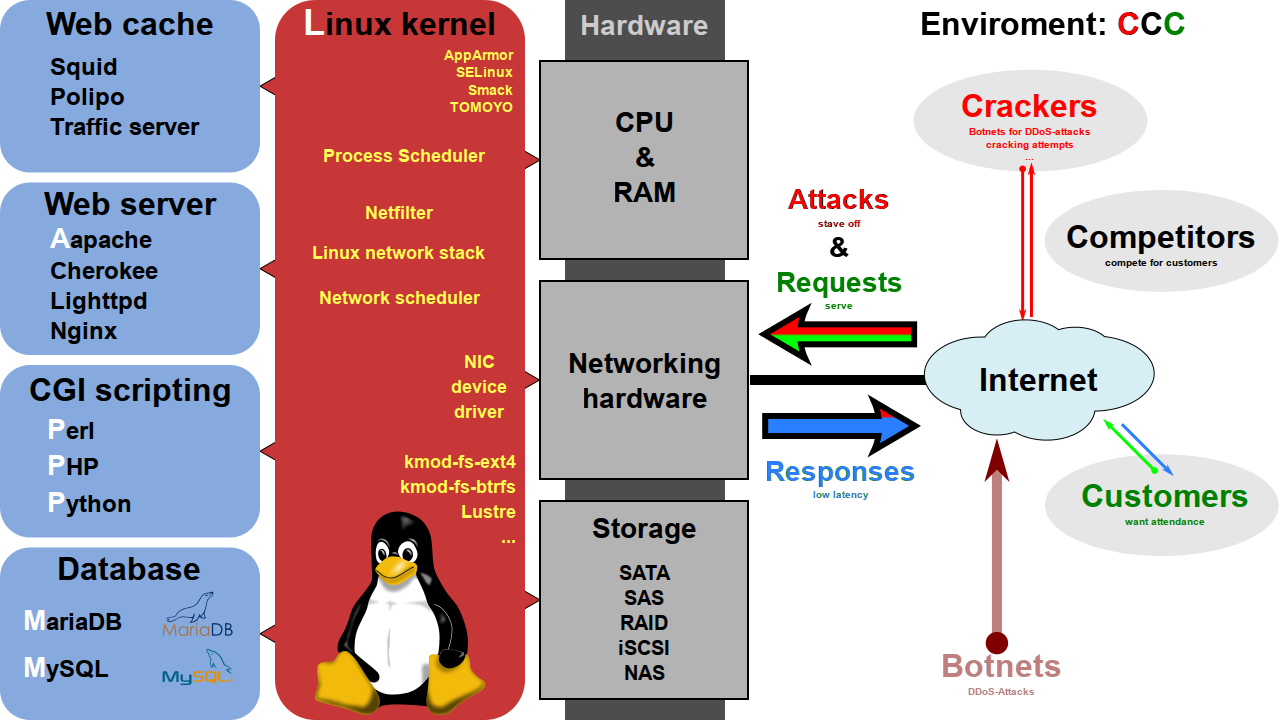
\includegraphics[scale=0.3]{LAMP_software_bundle.png}
\caption{The LAMP Architecture}
\label{LAMP_software_bundle}
\end{figure}

Broad overview of the LAMP software bundle, displayed here together with Squid. A high-performance and high-availability web server solution providing security in a hostile environment.

As of April 2007, over 20 million Internet domains had web services hosted on servers with PHP installed and \textcolor{Blue}{\texttt{mod\_php}} was recorded as the most popular Apache HTTP Server module.[94] PHP is used as the server-side programming language on 75\% of all websites whose server-side programming language is known, and PHP is the most-used open source software within enterprises. Web content management systems written in PHP include MediaWiki, Joomla, eZ Publish, SilverStripe, WordPress, Drupal, Moodle, the user-facing portion of Facebook, and Digg.

For specific and more advanced usage scenarios, PHP offers a well defined and documented way for writing custom extensions in C or C++. Besides extending the language itself in form of additional libraries, extensions are providing a way for improving execution speed where it is critical and there is room for improvements by using a true compiled language. PHP also offers well defined ways for embedding itself into other software projects. That way PHP can be easily used as an internal scripting language for another project, also providing tight interfacing with the project's specific internal data structures.

PHP是一个应用范围很广的语言,特别是在网络程序开发方面。一般来说PHP大多在服务器端运行,通过运行PHP的代码来产生网页提供浏览器读取,此外也可以用来开发命令行脚本程序和用户端的GUI应用程序。

PHP可以在许多的不同种的服务器、操作系统、平台上运行,也可以和许多数据库系统结合。使用PHP不需要任何费用,官方组织PHP Group提供了完整的程序源代码,允许用户修改、编译、扩充来使用。




\section{Frameworks}

PHP官方的框架为Zend framework,2005年开始开发至今已经步入成熟期,尽管对于PHP框架的方向业界还有争议,但在实际生产中框架的使用已非常普遍。

另一些常用的PHP框架有:Yii、CodeIgniter、CakePHP、Symfony、QeePHP/FleaPHP、ThinkPHP等,使用这些框架,可以使项目得到更快更简单的部署和更加敏捷的开发效率,但在另一方面,学习这些框架的使用需要付出额外的学习成本。





\section{Libraries}



内置多样化的函数是PHP主要的特点之一,这些开放代码的函数提供了各种不同的功能,例如文件处理、FTP、字符串处理、等等。这些函数的使用方法和C语言相近(例如printf),这也是PHP广为流行的原因之一。

除了内置的函数之外,PHP也提供了很多扩展库(extension),像是各种数据库连接函数、数据压缩函数、图形处理等等。有些延伸库需要从PECL(PHP Extension Community Library)取得。

以下是PHP编程语言提供的库列表。



\begin{table}
\centering
\caption{PHP Libraries}
\label{php_libraries}
\rowcolors{1}{White}{Lavender}
\begin{tabular}{m{65pt}m{135pt}m{90pt}m{80pt}}
Apache			&Gettext						&mSQL			&SESAM\\
BCMath			&GD Graphics Library			&MySQL		&Session Handling\\
Bzip2			&GNU Multi-Precision Library	&Mowhawk		&Shared memory\\
Calendars		&Hyperwave					&muscat		&SMTP\\
CCVS			&iconv							&Ncurses		&SNMP\\
COM			&IMAP,POP3 and NNTP		&ODBC			&Sockets\\
ClibPDF			&Informix						&Oracle		&SimpleXML\\
cURL			&Ingres II						&OpenSSL		&SQLite\\
Cybercash		&InterBase						&Ovrimos SQL	&Streams\\
DB2			&IRC							&PDF			&Sybase\\
dBase			&LDAP							&PayFlow Pro	&Token\\
DBM			&Lotus Notes					&PDO			&vpopmail\\
dbx				&mailparse						&POSIX			&WDDX\\
DB++			& MCAL							&PostgreSQL	&Win32 API\\
DOM XML		&Mcrypt						&Printer		&XML(Xpath)\\
.NET			&MCVE							&Pspell			&XML-RPC\\
FileMaker Pro	&Mhash							&GNU Readline	&XSLT\\
FrontBase		&MIME Functions				&GNU Recode	&YAZ\\
filePro			& MS-SQL						&Regular expressions&Yellow Pages/NIS\\
FriBiDi			&Ming							&QT-Dom		&ZIP\\
FTP				&mnoGoSearch					&Semaphores	&Zlib\\


\end{tabular}
\end{table}




\chapter{Security}


About 30\% of all vulnerabilities listed on the National Vulnerability Database are linked to PHP. These vulnerabilities are caused mostly by not following best-practice programming rules. Technical security flaws of the language itself or of its core libraries are not frequent (23 in 2008, about 1\% of the total). Recognizing that programmers make mistakes, some languages include taint checking to automatically detect the lack of input validation which induces many issues. Such a feature is being developed for PHP, but its inclusion in a release has been rejected several times in the past.

There are advanced protection patches such as Suhosin and Hardening-Patch, especially designed for web hosting environments.

Some of the vulnerabilities are induced by improper PHP's runtime configuration. For example, failing to disable PHP execution for the directory where uploaded images are stored, can result in execution of malicious PHP code embedded within uploaded images. Another well known example is leaving enabled the dynamic loading of PHP extensions, in a shared hosting environment.

据National Vulnerability Database数据显示,与PHP有关的数据库攻击比例为:20\% 2004, 28\% 2005, 43\% 2006, 36\% 2007, 35\% 2008 and 32\% 2009。其中很多的漏洞都可以通过远程操作完成,黑客可以通过网络连接攻击服务器,达到盗取或毁坏数据,发送垃圾邮件或进行分布式拒绝服务攻击。但是随着更多的关注,PHP也变得越来越安全了。


2010年12月17日,PHP代码“贡献者名单”中被加入“Wolegequ Gelivable”字样(中文含义“我勒个去 给力”),约半小时后被删除。2011年3月19日,PHP官方发布声明指出,黑客可能是通过wiki.php.net作为入口攻击了代码系统。并且,官方已经检查过自版本5.3.5以来发布的代码,并没有发现恶意内容。但官方同时表示,尚未完全掌握黑客发动本次攻击的具体细节。


\section{Thread Safe}

Windows版的PHP从版本5.2.1开始有Thread Safe(线程安全)和None Thread Safe(NTS,非线程安全)之分,这两者不同在于何处\cite{thread_safe}?到底应该用哪种?这里做一个简单的介绍。

从2000年10月20日发布的第一 个Windows版的PHP3.0.17开始的都是线程安全的版本。与Linux/Unix系统是采用多进程的工作方式不同的是,Windows系统的是多线程的工作方式。如果在IIS下以CGI方式运行PHP会非常慢,这是由于CGI模式是建立在多进程的基础之上的,而非多线程。

一般我们会把PHP配置成以ISAPI的方式来运行,ISAPI是多线程的方式,这样就快多了。但存在一个问题,很多常用的PHP扩展是以Linux/Unix的多进程思想来开发的,这些扩展在ISAPI的方式运行时就会出错搞垮IIS,因此在IIS下CGI模式才是PHP运行的最安全方式,但CGI模式对于每个HTTP请求都需要重新加载和卸载整个PHP环境,其消耗是巨大的。

为了兼顾IIS下PHP的效率和安全,微软给出了FastCGI的解决方案。FastCGI可以让PHP的进程重复利用而不是每一个新的请求就重开一个进程,同时FastCGI也可以允许几个进程同时执行。这样既解决了CGI进程模式消耗太大的问题,又利用上了CGI进程模式不存在线程安全问题的优势。

因此,如果是使用ISAPI的方式来运行PHP就必须用Thread Safe(线程安全)的版本;而用FastCGI模式运行PHP的话就没有必要用线程安全检查了,用None Thread Safe(NTS,非线程安全)的版本能够更好的提高效率。

\section{Version}

If you are using PHP with Apache 1 or Apache2 from apache.org you need to use the VC6 versions of PHP

If you are using PHP with IIS you should use the VC9 versions of PHP

VC6 Versions are compiled with the legacy Visual Studio 6 compiler

VC9 Versions are compiled with the Visual Studio 2008 compiler and have improvements in performance and stability. The VC9 versions require you to have the Microsoft 2008 C++ Runtime (x86) or the Microsoft 2008 C++ Runtime (x64) installed

Do NOT use VC9 version with apache.org binaries

VC9 versions of Apache can be fetched at Apache Lounge. We use their binaries to build the Apache SAPIs.







\chapter{Criticism}




PHP has been criticized for its heavy cluttering of main distribution with many functions, case-insensitive function names, among other specific details.


PHP has also been criticized heavily for the security vulnerabilities that can be created by certain language features, induced by some of the historically default values for their associated runtime settings. Among these, magic quotes and \textcolor{Blue}{\texttt{register\_globals}} are the best known. The latter made any URL parameters become variables, which while making programming easier, could create serious security vulnerabilities as it allowed an attacker to set the value of any variable and interfere with script execution.

It is felt PHP interferes with productivity because the lack of language design introduces unpredictable behavior, inconsistent function naming and parameter usage, dependency on new constructs to work around lower level language quirks, introduction of new constructs with flaky behavior, and missing or inconsistent error handling features.


It also lacks features such as native Unicode support and multithreading at the PHP core level, though using threads is made possible by the pthreads PECL extension.



\bibliographystyle{plainnat}
\bibliography{phpnotes}
\setcitestyle{numbers}
















































































\end{document}


























